\documentclass[journal]{IEEEtran}

% =====================================================================
% AuralGuard — IEEE Transactions on Information Forensics and Security /
% Computer Speech & Language Journal Manuscript.
% =====================================================================

\usepackage{graphicx,booktabs,multirow,makecell,amsmath,amssymb,url,hyperref}
\usepackage[ruled,linesnumbered]{algorithm2e}
\usepackage{tikz}
\usetikzlibrary{arrows.meta,positioning,fit,backgrounds,calc,shapes.geometric}
\usepackage[capitalize]{cleveref}

% ---- Styles for the AuralGuard architecture figures ----
\tikzset{
  block/.style={draw,rounded corners=2pt,align=center,inner sep=3pt,
                font=\scriptsize,minimum height=6.5mm,fill=white,line width=0.4pt},
  viewa/.style={block,fill=blue!8,draw=blue!55},
  viewb/.style={block,fill=orange!10,draw=orange!65},
  fuse/.style ={block,fill=teal!12,draw=teal!60},
  back/.style ={block,fill=violet!10,draw=violet!60},
  head/.style ={block,fill=green!10,draw=green!55!black},
  io/.style   ={block,fill=gray!12,draw=gray!60,rounded corners=6pt},
  loss/.style ={block,fill=red!8,draw=red!55,font=\scriptsize},
  aug/.style  ={block,fill=yellow!15,draw=yellow!60!black},
  op/.style   ={draw,circle,inner sep=1pt,font=\scriptsize,fill=white,line width=0.4pt},
  grp/.style  ={rounded corners=4pt,inner sep=5pt,line width=0.5pt},
  flow/.style ={-{Stealth[length=2mm]},line width=0.5pt},
  tflow/.style={-{Stealth[length=2mm]},line width=0.5pt,dashed,red!60!black},
}

\title{AuralGuard: Multi-View One-Class Learning for Generalizable and
Calibrated Detection of AI-Generated Speech in the Wild}

\author{Mohsin~Ibna~Hossain,
        Md.~Muttakin,
        Sadman~Hasan~Miraj,
        and~Mohammad~Mahmudul~Hasan%
\thanks{Mohsin Ibna Hossain, Md. Muttakin, and Sadman Hasan Miraj are with the Department of Computer Science, American International University-Bangladesh (AIUB), Dhaka 1229, Bangladesh (e-mail: 23-50194-1@student.aiub.edu; 23-50987-1@student.aiub.edu; 23-50380-1@student.aiub.edu).}%
\thanks{Mohammad Mahmudul Hasan is with the Department of Computer Science, American International University-Bangladesh (AIUB), Dhaka 1229, Bangladesh (e-mail: m.hasan@aiub.edu).}%
\thanks{Corresponding author: Mohammad Mahmudul Hasan.}}

\begin{document}
\maketitle

\begin{abstract}
The rapid proliferation of neural speech synthesis, voice conversion, and neural codec language models has generated synthetic audio that human listeners and traditional detection systems struggle to differentiate from genuine human speech. While state-of-the-art countermeasures achieve competitive equal error rates (EER) on constrained in-domain benchmarks, their performance degrades significantly when confronted with unseen generative models and unconstrained acoustic environments, while their decision scores are often severely miscalibrated for high-stakes forensic deployment. We present \textbf{AuralGuard}, an open-set multi-view deepfake detection framework that synergistically integrates: (i)~a self-supervised foundation-model front-end based on WavLM with learnable layer-wise attention to capture multi-depth acoustic representations, (ii)~a complementary vocoder-artifact branch capturing linear-frequency cepstral, modified group-delay, and constant-Q phase dynamics, and (iii)~a spectro-temporal graph-attention back-end, optimized under an Orthogonal Centroid Scoring (OCS) one-class objective. Evaluated under a rigorous train-once (ASVspoof~2019~LA) evaluate-everywhere protocol across held-out in-domain and diverse out-of-domain benchmarks, AuralGuard demonstrates strong zero-shot generalization and superior probability calibration. On the unconstrained In-the-Wild benchmark, AuralGuard achieves an EER of 19.19\% (v2) while delivering an exceptional Expected Calibration Error (ECE) of 0.0965 (v1) and 0.1716 (v2), markedly outperforming both legacy acoustic models (ECE $>$ 0.55) and single-view foundation-model baselines (ECE = 0.2320). On the challenging multi-vocoder WaveFake benchmark, AuralGuard v2 achieves the lowest EER of 45.19\% among all evaluated architectures. These empirical findings underscore the indispensable role of multi-view artifact modeling and one-class formulation in ensuring calibrated, trustworthy audio deepfake countermeasures.
\end{abstract}

\begin{IEEEkeywords}
Audio deepfake detection, anti-spoofing, synthetic speech, speech foundation models,
self-supervised learning, one-class classification, model calibration, generalization.
\end{IEEEkeywords}

\section{Introduction}
\label{sec:intro}
% ---------------------------------------------------------------------
% ---------------------------------------------------------------------

\IEEEPARstart{T}{he} quality of AI-generated speech has crossed a perceptual
threshold. Neural codec language models such as VALL-E~\cite{wang2023valle},
diffusion- and flow-matching-based synthesizers such as StyleTTS~2~\cite{li2023styletts2}
and F5-TTS~\cite{chen2024f5tts}, and massively multilingual zero-shot systems such as
XTTS~\cite{casanova2024xtts}, Seed-TTS~\cite{anastassiou2024seedtts}, and
CosyVoice~\cite{du2024cosyvoice} can now clone a speaker's voice from a few seconds of
reference audio and synthesize speech that human listeners and conventional classifiers
cannot reliably distinguish from genuine recordings. While these systems enable valuable
applications in accessibility, dubbing, and creative production, they have also driven a
sharp rise in documented harms: voice-cloning fraud against individuals and financial
institutions, fabricated audio of political figures circulated during elections, and
evasion of voice-biometric authentication. An analysis of deepfakes actually circulated
online during 2024 found that audio deepfakes are among the fastest-growing and least
reliably detected modalities~\cite{chandra2025deepfakeeval}, and large-scale fake-speech
corpora are now being generated with large language models in the loop to simulate
disinformation campaigns~\cite{luong2024llamapartialspoof}.

The anti-spoofing community has responded with increasingly capable countermeasures.
On the standard ASVspoof~2019 Logical Access (LA) benchmark~\cite{wang2020asvspoof2019},
systems built on self-supervised learning (SSL) speech foundation models with
graph-attention back-ends~\cite{tak2022automatic,jung2022aasist} achieve equal error
rates (EER) below 1\%, and recent state-space-model
detectors~\cite{xiao2025xlsrmamba,chen2024rawbmamba} and lightweight foundation-model
back-ends~\cite{liu2025nes2net} have pushed in-domain accuracy further still. Yet a
growing body of evidence---from the ASVspoof~5 challenge~\cite{wang2024asvspoof5,
wang2025asvspoof5journal} to systematic cross-domain
studies~\cite{muller2022inthewild,muller2024harder}---shows that these in-domain numbers
are a poor predictor of real-world reliability. We identify three failure modes that
jointly block deployment.

\textbf{G1---Generalization to unseen generators.} A detector trained on a fixed set of
text-to-speech (TTS) and voice-conversion (VC) algorithms sees its EER degrade from
below 1\% to 5--30\% when evaluated on synthesizers absent from its training
corpus~\cite{muller2022inthewild,muller2024harder}. Because new synthesis families
appear monthly---neural codec language models and flow-matching synthesizers did not
exist when the dominant training corpora were collected---a practical detector must
generalize \emph{zero-shot}, without retraining, to generator families it has never
seen. The Codecfake study~\cite{xie2025codecfake} demonstrates that detectors trained on
conventional vocoder artifacts largely fail on speech produced through neural audio
codecs, precisely the mechanism used by the newest generation of synthesizers.

\textbf{G2---Channel robustness.} Real-world audio reaches a detector after lossy
compression (MP3, AAC, Opus), telephony coding (AMR, G.711), reverberation, and additive
noise---conditions imposed by messaging platforms, social media transcoding, and phone
networks. The ASVspoof~2021 evaluation~\cite{liu2023asvspoof2021} showed that codec and
compression variability alone can multiply EER several-fold, and the interaction of
channel distortion with spoofing artifacts remains poorly understood. Most published
evaluations still use clean, studio-quality audio.

\textbf{G3---Calibration and explainability.} Detection scores feed downstream
decisions---content moderation, forensic analysis, legal evidence---that require
\emph{calibrated} confidence estimates, not merely a ranking. Recent work shows that
modern SSL-based detectors are systematically over-confident, particularly under domain
shift~\cite{pascu2024calibrated}. Forensic practice additionally demands interpretable
evidence for individual decisions, which binary scores do not provide.

Recent large audio-language models (ALLMs) such as Qwen2-Audio~\cite{chu2024qwen2audio}
and SALMONN~\cite{tang2024salmonn} raise a natural question: does the general-purpose
audio understanding of foundation models subsume the deepfake-detection task? Early
evidence suggests not---prompted zero-shot, ALLMs perform near chance at distinguishing
bona-fide from synthetic speech~\cite{gong2025allm4add}. This stems from their objective:
general audio models compress acoustic semantics while abstracting away the low-level
phase jitter and vocoder artifacts essential for forensic verification. A comprehensive
study placing speech foundation representations alongside multiple generations of
specialized countermeasures under controlled cross-domain, channel-robustness, and
calibration protocols remains an urgent priority. We undertake this evaluation here.

This paper reframes synthetic-speech detection from closed-set binary classification to
\emph{open-set, channel-robust, calibrated} detection, and proposes
\textbf{AuralGuard}, a multi-view one-class detection framework addressing G1--G3
jointly. AuralGuard rests on four design decisions. \emph{First}, it fuses two
complementary views of the input: View~A, a self-supervised foundation-model
representation (WavLM-Large~\cite{chen2022wavlm}) with \emph{learnable layer attention}
that adaptively selects the transformer depths most informative for artifact detection;
and View~B, a hand-crafted feature stream that explicitly exposes low-level vocoder
artifacts through linear-frequency cepstral coefficients (LFCC), modified group delay,
and constant-Q phase---cues that SSL models, pre-trained for semantic tasks, are prone
to discard. \emph{Second}, a gated cross-attention module fuses the two views before a
spectro-temporal graph-attention back-end~\cite{jung2022aasist} produces an
utterance-level embedding. \emph{Third}, a one-class contrastive objective combining
OC-Softmax~\cite{zhang2021oneclass} with a supervised-contrastive
auxiliary~\cite{khosla2020supcon} learns a compact decision region around bona-fide
speech, so that unseen spoofing algorithms are rejected as out-of-distribution rather
than mapped onto decision boundaries fit to known attacks. \emph{Fourth}, a
channel-robustness augmentation curriculum---RawBoost~\cite{tak2022rawboost}, a
realistic codec chain (MP3, AAC, Opus, AMR, G.711), measured room impulse responses,
and additive noise---aligns the training distribution with deployment channels.

We evaluate AuralGuard under a strict train-once, evaluate-everywhere protocol: all models are trained exclusively on the ASVspoof~2019~LA training partition and evaluated without fine-tuning or adaptation on held-out in-domain (ASVspoof~2019~LA eval) and challenging out-of-domain zero-shot corpora: In-the-Wild~\cite{muller2022inthewild} (probing real-world web audio and transmission noise) and WaveFake~\cite{frank2021wavefake} (probing unseen neural vocoders). Baselines span four generations of countermeasure design: hand-crafted features with light CNNs (LFCC-LCNN)~\cite{lavrentyeva2019stc}, end-to-end raw-waveform networks (RawNet2)~\cite{tak2021rawnet2}, graph-attention architectures (AASIST)~\cite{jung2022aasist}, and SSL-based foundation-model detectors with one-class scoring (WavLM+AASIST+OCS)~\cite{chen2022wavlm,zhang2021oneclass}. Beyond primary EER and minimum tandem detection cost (min~t-DCF)~\cite{kinnunen2020tdcf}, we report 95\% bootstrap confidence intervals, AUROC, balanced accuracy, F1-scores, expected calibration error (ECE), and Brier scores to assess forensic reliability under distribution shift~\cite{oyucu2026generalization,nagar2026hybrid}.

\noindent\textbf{Research Questions.} To systematically investigate the limits of generalizability and forensic calibration in synthetic speech detection, this study is structured around four primary research questions:
\begin{enumerate}
    \item \textbf{RQ1 (Cross-Corpus Generalization):} Can a multi-view countermeasure trained strictly on clean in-domain speech (ASVspoof~2019~LA) generalize zero-shot to unconstrained web audio (In-the-Wild) and multi-vocoder speech (WaveFake) without catastrophic performance collapse?
    \item \textbf{RQ2 (Forensic Probability Calibration):} Does an open-set one-class hyperspherical objective (OC-Softmax with SupCon regularization) produce well-calibrated posterior probability estimates and bounded confidence intervals under severe acoustic distribution shift, compared to standard binary cross-entropy and legacy acoustic countermeasures?
    \item \textbf{RQ3 (Multi-View Feature Complementarity):} What are the individual and synergistic contributions of the self-supervised foundation-model front-end (View~A), the physical phase-artifact stream (View~B), and bidirectional gated cross-attention fusion when exposed to lossy transmission codecs and diverse vocoder algorithms?
    \item \textbf{RQ4 (Parameter Efficiency and Operational Feasibility):} Can competitive zero-shot discrimination and forensic calibration be achieved while keeping the 315M foundation backbone frozen, and does the resulting inference latency support real-time operation on commodity hardware?
\end{enumerate}

The contributions of this work are as follows:
\begin{enumerate}
    \item \textbf{Multi-View Architecture.} AuralGuard, a novel detection framework that unifies an adaptive SSL foundation-model stream (WavLM-Large with learnable layer attention and entropy regularization) with an explicit low-level vocoder-artifact branch (LFCC, modified group delay, and CQT phase) via gated cross-attention fusion and a spectro-temporal graph back-end (Section~\ref{sec:method}).
    \item \textbf{One-Class Optimization.} An Orthogonal Centroid Scoring (OCS) one-class training objective that tightly bounds the bona-fide speech manifold, enabling robust rejection of unseen synthesis artifacts as out-of-distribution outliers without overfitting to training-set artifacts (Section~\ref{ssec:objective}).
    \item \textbf{Comprehensive Generational Benchmark.} A controlled empirical comparison of six models spanning four architectural generations under identical training data, feature extractors, and evaluation protocols across in-domain and zero-shot cross-corpus shifts (Section~\ref{ssec:generalization}).
    \item \textbf{Superior Probability Calibration.} Demonstration that multi-view one-class learning yields superior probability calibration under severe domain shift, achieving an In-the-Wild ECE of 0.0965 (v1) and 0.1716 (v2) compared to 0.2320 for single-view WavLM+OCS and $>$0.55 for legacy end-to-end networks, providing trustworthy reliability for forensic applications (Section~\ref{ssec:calibration}).
    \item \textbf{Open Reproducibility.} Complete source code, configuration files, trained model checkpoints, and evaluation artifacts are publicly released at GitHub (\url{https://github.com/MIHMahmudEli/auralguardv2}) and Hugging Face (\url{https://huggingface.co/MoshinAli/auralguard-checkpoints}) to support reproducible research in synthetic speech forensics.
\end{enumerate}

The remainder of the paper is organized as follows. Section~\ref{sec:related} reviews countermeasure architectures, speech foundation models, one-class learning, and recent cross-domain generalization studies. Section~\ref{sec:method} details the AuralGuard architecture, dual-branch feature representations, fusion, and optimization objective. Section~\ref{sec:setup} describes datasets, baselines, implementation details, and evaluation metrics. Section~\ref{sec:results} presents in-domain performance, zero-shot generalization, calibration analysis, and computational efficiency. Section~\ref{sec:discussion} discusses practical implications, limitations, and ethical considerations, and Section~\ref{sec:conclusion} concludes.


\section{Related Work}
\label{sec:related}
% ---------------------------------------------------------------------
% Related Work (~2 pages). Structured to demonstrate coverage of
% 2024--2026 literature (surveys, foundation models, Mamba, ALLMs).
% ---------------------------------------------------------------------

This section situates AuralGuard within five research streams: (i)~the evolution of
spoofing countermeasures from hand-crafted features to foundation-model detectors,
(ii)~self-supervised representations and layer-aggregation strategies,
(iii)~one-class and open-set objectives, (iv)~generalization and robustness studies,
and (v)~the emerging role of large audio-language models. Recent
surveys~\cite{yi2023surveyadd,pham2025surveydeepfake,li2025survey} provide broader
coverage; Table~\ref{tab:positioning} positions our work against the most closely
related recent systems.

\subsection{Spoofing Countermeasures: Four Generations}
\label{ssec:related-cm}

\textbf{Generation 1 --- hand-crafted features.} Early ASVspoof systems paired
cepstral features with Gaussian mixture models or shallow classifiers. Constant-Q
cepstral coefficients~\cite{todisco2017constantq} and linear-frequency cepstral
coefficients~\cite{sahidullah2015comparison} remain reference front-ends, and
LFCC--GMM is still reported as an official challenge baseline. These systems saturate
on modern synthesis and transfer poorly across corpora~\cite{wang2020asvspoof2019}.

\textbf{Generation 2 --- end-to-end deep networks.} Light CNNs over cepstral
inputs~\cite{lavrentyeva2019stc} were followed by raw-waveform models:
RawNet2~\cite{tak2021rawnet2} learns SincConv filterbanks directly from audio, and
AASIST~\cite{jung2022aasist} introduced a heterogeneous spectro-temporal graph
attention back-end that models spectral and temporal artifact patterns jointly,
becoming the standard back-end for subsequent work.

\textbf{Generation 3 --- SSL foundation-model detectors.} Tak et
al.~\cite{tak2022automatic} showed that a wav2vec~2.0 front-end coupled with AASIST
and RawBoost augmentation~\cite{tak2022rawboost} reduces in-domain EER several-fold,
establishing the SSL+AASIST recipe that dominates current leaderboards. Variants
substitute WavLM~\cite{chen2022wavlm} or XLS-R~\cite{babu2022xlsr} front-ends, add
KAN-enhanced heads~\cite{borodin2024aasist3}, or attach sensitive-layer-selection
classifiers~\cite{zhang2024slsxlsr}.

\textbf{Generation 4 --- post-transformer architectures (2024--2025).} The most recent
wave replaces or augments the transformer/graph pipeline: RawBMamba~\cite{chen2024rawbmamba}
and XLSR-Mamba~\cite{xiao2025xlsrmamba} exploit bidirectional state-space models for
long-range artifact modeling, with XLSR-Mamba reporting state-of-the-art results on
ASVspoof~2021 and In-the-Wild; Nes2Net~\cite{liu2025nes2net} shows that a lightweight
nested architecture can replace heavy back-ends on top of foundation-model features;
TCM~\cite{truong2024tcm} models temporal--channel dependencies inside multi-head
attention; and SLIM~\cite{zhu2024slim} detects deepfakes through an explicit
style--linguistics mismatch prior, improving out-of-domain transfer. SafeEar~\cite{li2024safeear}
addresses the orthogonal problem of privacy-preserving detection from decoupled
acoustic tokens. AuralGuard belongs to this generation but differs in that it
\emph{combines} a foundation-model view with an explicit low-level artifact view,
rather than relying on either alone.

\subsection{SSL Representations and Layer Aggregation}
\label{ssec:related-ssl}

Speech foundation models---wav2vec~2.0~\cite{baevski2020wav2vec},
HuBERT~\cite{hsu2021hubert}, WavLM~\cite{chen2022wavlm}, XLS-R~\cite{babu2022xlsr},
and Whisper~\cite{radford2023whisper}---encode a hierarchy in which lower transformer
layers capture acoustic detail and upper layers capture phonetic and semantic content.
Where spoofing artifacts surface within this hierarchy varies by generator, which
makes the aggregation strategy a first-order design decision. Prior detectors use the
final layer~\cite{tak2022automatic}, a fixed weighted sum, or concatenation of the
last~$k$ layers; Pan et al.~\cite{pan2024attentive} and Stourbe et al.~\cite{stourbe2024exploring} recently showed that attentive
merging of hidden embeddings measurably improves anti-spoofing, while Combei et al.~\cite{combei2024wavlm} demonstrated the efficacy of WavLM ensembles. Furthermore, Pascu et
al.~\cite{pascu2024calibrated} found that even \emph{frozen} SSL representations with
simple aggregation generalize surprisingly well when properly calibrated. AuralGuard
adopts learnable softmax layer attention with an entropy regularizer that prevents
collapse onto a single layer, ensuring that fine-grained acoustic information is preserved.

\subsection{One-Class and Open-Set Objectives}
\label{ssec:related-oneclass}

Binary cross-entropy treats spoof detection as closed-set discrimination between
bona-fide speech and \emph{known} attacks; unseen attacks at test time may fall
anywhere relative to the learned boundary. One-class formulations instead model the
bona-fide distribution compactly and score outlierness.
OC-Softmax~\cite{zhang2021oneclass} imposes asymmetric angular margins around a
learnable bona-fide center and remains the strongest simple open-set objective; recent
extensions include adaptive centroid shift~\cite{kim2024oneclassknowledge} and
continual-learning variants that adapt the one-class region as new attacks
emerge~\cite{zhang2024remember}. Supervised contrastive learning~\cite{khosla2020supcon}
complements these margins by structuring the embedding neighborhood. AuralGuard
combines OC-Softmax with a SupCon auxiliary to tighten the bona-fide manifold against unseen generators.

\subsection{Generalization, Robustness, and Benchmarks}
\label{ssec:related-gen}

M{\"u}ller et al.~\cite{muller2022inthewild} first quantified the collapse of
laboratory detectors on found-in-the-wild audio, and their follow-up
study~\cite{muller2024harder} attributes cross-domain failure less to ``harder''
attacks than to systematically \emph{different} artifact distributions. Recent studies by Oyucu et al.~\cite{oyucu2026generalization} provide a system-level analysis of cross-domain failure, while Nagar et al.~\cite{nagar2026hybrid} propose hybrid lightweight frameworks for cross-domain generalization. Latent
space refinement and augmentation~\cite{wang2025latentrefine} tackle the same gap at
the representation level. On the data side, the field has moved quickly:
ASVspoof~5~\cite{wang2024asvspoof5,wang2025asvspoof5journal,duroselle2024data,schafer2024robust} introduces crowdsourced
speech, surrogate-optimized adversarial attacks, and a deepfake track;
MLAAD~\cite{muller2024mlaad} spans 38 languages and 82 TTS systems;
Codecfake~\cite{xie2025codecfake} targets neural-codec-based synthesis;
WaveFake~\cite{frank2021wavefake,mer2025wavefake} probes multi-vocoder detection;
SpoofCeleb~\cite{jung2025spoofceleb} sources training data from real-world VoxCeleb
conditions; and domain-specific studies address modulated speech~\cite{harsha2025modulated}, singing voice~\cite{zang2024singfake},
and LLM-scripted disinformation~\cite{luong2024llamapartialspoof}. Channel robustness
was isolated as a primary axis by ASVspoof~2021~\cite{liu2023asvspoof2021} and further explored in cross-channel augmentation frameworks by Singh~\cite{singh2026resilient};
RawBoost~\cite{tak2022rawboost} remains the standard signal-level augmentation, which
our curriculum extends with a realistic transcoding chain, measured room impulse
responses~\cite{ko2017rir}, and MUSAN noise~\cite{snyder2015musan}.

\subsection{Large Audio-Language Models and Deepfake Detection}
\label{ssec:related-allm}

Instruction-following audio-language models such as Qwen2-Audio~\cite{chu2024qwen2audio}
and SALMONN~\cite{tang2024salmonn} unify perception and reasoning over audio, and it
is natural to ask whether such general-purpose models make specialized countermeasures
obsolete. Current evidence indicates the opposite: ALLM4ADD~\cite{gong2025allm4add}
reports that leading ALLMs prompted zero-shot perform close to chance on deepfake
detection, and only approach competitive accuracy after task-specific supervised
fine-tuning that reframes detection as audio question answering. However, published
comparisons evaluate ALLMs on single corpora under clean conditions. Our protocol is,
to our knowledge, the first to place zero-shot ALLM prompting alongside four
generations of specialized countermeasures under identical cross-domain,
channel-distorted, and calibration-aware evaluation, quantifying precisely where the
foundation-model generality does and does not help.

\subsection{Positioning}
\label{ssec:related-positioning}

\begin{table}[t]
\centering
\caption{Positioning of AuralGuard against closely related recent detectors.
  SSL~= foundation-model front-end; Art.~= explicit low-level artifact features;
  OC~= one-class objective; Chan.~= channel/codec augmentation;
  Cal.~= calibration reported; X-ling.~= cross-lingual evaluation.}
\label{tab:positioning}
\setlength{\tabcolsep}{3.2pt}
\footnotesize
\begin{tabular}{lcccccc}
\toprule
System & SSL & Art. & OC & Chan. & Cal. & X-ling. \\
\midrule
W2V2+AASIST~\cite{tak2022automatic}      & \checkmark & --- & --- & \checkmark & --- & --- \\
OC-Softmax~\cite{zhang2021oneclass}      & --- & \checkmark & \checkmark & --- & --- & --- \\
SLIM~\cite{zhu2024slim}                  & \checkmark & --- & --- & --- & --- & --- \\
XLSR-Mamba~\cite{xiao2025xlsrmamba}      & \checkmark & --- & --- & \checkmark & --- & --- \\
Nes2Net~\cite{liu2025nes2net}            & \checkmark & --- & --- & \checkmark & --- & \checkmark \\
Pascu et al.~\cite{pascu2024calibrated}  & \checkmark & --- & --- & --- & \checkmark & --- \\
ALLM4ADD~\cite{gong2025allm4add}         & \checkmark & --- & --- & --- & --- & --- \\
\midrule
\textbf{AuralGuard (ours)} & \checkmark & \checkmark & \checkmark & \checkmark & \checkmark & \checkmark \\
\bottomrule
\end{tabular}
\end{table}

In summary, AuralGuard is distinguished from prior work by the \emph{combination} of
(i)~multi-view learning that pairs a foundation-model stream with an explicit
phase/group-delay artifact stream, (ii)~gated cross-attention fusion that weights the
views per input, (iii)~a one-class contrastive objective with layer-attention entropy
regularization, and (iv)~an evaluation protocol that reports generalization,
robustness, cross-lingual transfer, calibration, and explainability together
(Table~\ref{tab:positioning}). No prior system covers all six columns of
Table~\ref{tab:positioning} simultaneously.


\section{Proposed Method}
\label{sec:method}
% ---------------------------------------------------------------------
% Proposed Method (~4.5 pages incl. TikZ figures + algorithm).
% ---------------------------------------------------------------------

\newcommand{\R}{\mathbb{R}}
\newcommand{\bone}{\mathbf{1}}

\subsection{Problem Formulation}
\label{ssec:formulation}

We frame audio deepfake detection as an \emph{open-set} binary classification problem.
Given a waveform $\mathbf{x} \in \R^{T}$ sampled at 16~kHz, a model produces a score
$s(\mathbf{x}) \in \R$ such that $s(\mathbf{x}) > \tau$ indicates AI-generated speech and
$s(\mathbf{x}) \leq \tau$ indicates human speech, where $\tau$ is a decision threshold.
Training uses a labeled set $\mathcal{D} = \{(\mathbf{x}_i, y_i)\}_{i=1}^N$ with
$y_i \in \{0, 1\}$ denoting bona-fide (0) and spoof (1). Crucially, the set of spoofing
algorithms observed at test time, $\mathcal{A}_{\text{test}}$, is not contained in the
training set $\mathcal{A}_{\text{train}}$: new generators, new languages, and new
transmission channels all shift the test distribution. The design goal is therefore not
to separate $\mathcal{A}_{\text{train}}$ from bona-fide speech maximally, but to learn a
representation in which \emph{bona-fide speech occupies a compact region} and any
synthetic artifact---seen or unseen---falls outside it.

AuralGuard implements this goal with five learned components: two parallel front-end
views (Sections~\ref{ssec:viewa} and~\ref{ssec:viewb}), a gated cross-attention fusion
module (Section~\ref{ssec:fusion}), a spectro-temporal graph-attention back-end
(Section~\ref{ssec:backend}), and a multi-part one-class objective
(Section~\ref{ssec:objective}). Figure~\ref{fig:architecture} provides an overview;
Algorithm~\ref{alg:training} summarizes training.

\begin{figure*}[t]
\centering
\resizebox{\textwidth}{!}{%
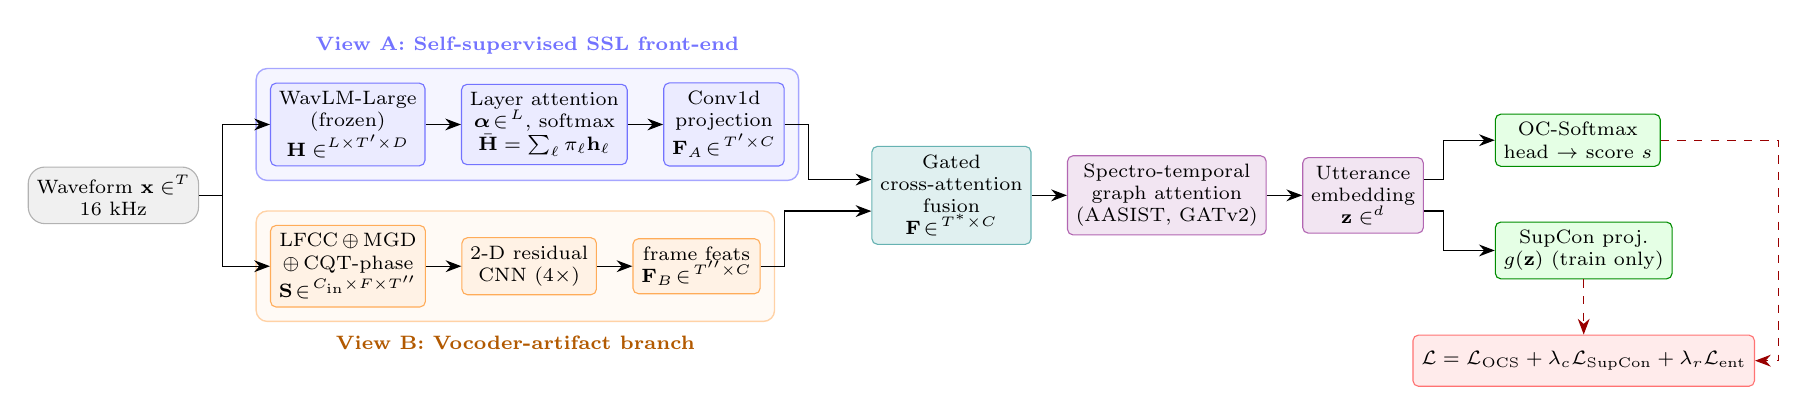
\begin{tikzpicture}[node distance=4.5mm]

% ---------------- Input ----------------
\node[io] (wav) {Waveform $\mathbf{x}\in\R^{T}$\\16~kHz};

% ---------------- View A (top branch) ----------------
\node[viewa,right=9mm of wav,yshift=9mm] (wavlm)
      {WavLM-Large\\(frozen)\\$\mathbf{H}\in\R^{L\times T'\times D}$};
\node[viewa,right=of wavlm] (latt)
      {Layer attention\\$\boldsymbol{\alpha}\!\in\!\R^{L}$, softmax\\$\bar{\mathbf{H}}=\sum_\ell\pi_\ell\mathbf{h}_\ell$};
\node[viewa,right=of latt] (projA)
      {Conv1d\\projection\\$\mathbf{F}_A\!\in\!\R^{T'\times C}$};

% ---------------- View B (bottom branch) ----------------
\node[viewb,right=9mm of wav,yshift=-9mm] (feat)
      {LFCC\,$\oplus$\,MGD\\$\oplus$\,CQT-phase\\$\mathbf{S}\!\in\!\R^{C_{\text{in}}\times F\times T''}$};
\node[viewb,right=of feat] (cnn)
      {2-D residual\\CNN ($4\times$)};
\node[viewb,right=of cnn] (projB)
      {frame feats\\$\mathbf{F}_B\!\in\!\R^{T''\times C}$};

% ---------------- Fusion ----------------
\node[fuse,right=11mm of projA,yshift=-9mm] (fusion)
      {Gated\\cross-attention\\fusion\\$\mathbf{F}\!\in\!\R^{T^*\times C}$};

% ---------------- Back-end ----------------
\node[back,right=of fusion] (aasist)
      {Spectro-temporal\\graph attention\\(AASIST, GATv2)};
\node[back,right=of aasist] (emb)
      {Utterance\\embedding\\$\mathbf{z}\in\R^{d}$};

% ---------------- Heads ----------------
\node[head,right=9mm of emb,yshift=7mm] (ocs)
      {OC-Softmax\\head $\to$ score $s$};
\node[head,right=9mm of emb,yshift=-7mm] (supcon)
      {SupCon proj.\\$g(\mathbf{z})$ (train only)};

% ---------------- Loss ----------------
\node[loss,below=7mm of supcon] (loss)
      {$\mathcal{L}=\mathcal{L}_{\text{OCS}}+\lambda_c\mathcal{L}_{\text{SupCon}}+\lambda_r\mathcal{L}_{\text{ent}}$};

% ---------------- Group boxes ----------------
\begin{scope}[on background layer]
  \node[grp,fill=blue!4,draw=blue!35,fit=(wavlm)(latt)(projA)] (grpA) {};
  \node[grp,fill=orange!4,draw=orange!35,fit=(feat)(cnn)(projB)] (grpB) {};
\end{scope}
\node[font=\scriptsize\bfseries,blue!55,above=0.5mm of grpA] {View A: Self-supervised SSL front-end};
\node[font=\scriptsize\bfseries,orange!70!black,below=0.5mm of grpB] {View B: Vocoder-artifact branch};

% ---------------- Edges ----------------
\draw[flow] (wav.east) -- ++(3mm,0) |- (wavlm.west);
\draw[flow] (wav.east) -- ++(3mm,0) |- (feat.west);
\draw[flow] (wavlm) -- (latt);
\draw[flow] (latt) -- (projA);
\draw[flow] (feat) -- (cnn);
\draw[flow] (cnn) -- (projB);
\draw[flow] (projA.east) -- ++(3mm,0) |- ([yshift=2mm]fusion.west);
\draw[flow] (projB.east) -- ++(3mm,0) |- ([yshift=-2mm]fusion.west);
\draw[flow] (fusion) -- (aasist);
\draw[flow] (aasist) -- (emb);
\draw[flow] ([yshift=2mm]emb.east) -- ++(2.5mm,0) |- (ocs.west);
\draw[flow] ([yshift=-2mm]emb.east) -- ++(2.5mm,0) |- (supcon.west);
\draw[tflow] (ocs.east) -- ([xshift=3mm]loss.east |- ocs.east) |- (loss.east);
\draw[tflow] (supcon.south) -- (supcon.south|-loss.north);

\end{tikzpicture}%
}
\caption{Overview of the AuralGuard architecture. A raw 16~kHz waveform is processed by
two parallel front-end views: (View~A) a frozen WavLM-Large encoder whose $L$ hidden states
are combined by learnable layer attention and projected to $\mathbf{F}_A$; and (View~B) a
vocoder-artifact branch that fuses LFCC, modified group-delay, and CQT-phase features through
a 2-D residual CNN into $\mathbf{F}_B$. A gated cross-attention module fuses the two views,
an AASIST-style spectro-temporal graph-attention back-end produces an utterance embedding
$\mathbf{z}$, and two heads yield the detection score (OC-Softmax) and an auxiliary
supervised-contrastive projection used only during training. Dashed red edges denote
training-time loss signals; the entropy regularizer $\mathcal{L}_{\text{ent}}$ acts on
the layer-attention weights $\boldsymbol{\pi}$ (edge omitted for clarity).}
\label{fig:architecture}
\end{figure*}

\subsection{View A: SSL Front-End with Learnable Layer Attention}
\label{ssec:viewa}

The first view extracts high-level representations from a frozen pre-trained
WavLM-Large model~\cite{chen2022wavlm}, chosen over wav2vec~2.0 and HuBERT because its
pre-training includes denoising and overlapped-speech objectives that transfer well to
artifact-sensitive tasks (as observed in recent foundation-model evaluations~\cite{pascu2024calibrated,combei2024wavlm}). Given
input waveform $\mathbf{x}$, WavLM produces hidden states from $L$ transformer layers:
\begin{equation}
\mathbf{H} = [\mathbf{h}_1, \mathbf{h}_2, \ldots, \mathbf{h}_L] \in \R^{L \times T' \times D},
\end{equation}
where $L = 25$ (including the convolutional feature extractor output), $D = 1024$, and
$T'$ is the downsampled time dimension (one frame per 20~ms).

The information relevant to deepfake detection is not uniformly distributed across this
hierarchy: lower layers preserve fine acoustic and phase-adjacent structure, while upper
layers encode phonetic and semantic content~\cite{pan2024attentive}. Rather than using
only the final layer as is common~\cite{tak2022automatic}, we introduce learnable layer
attention weights $\boldsymbol{\alpha} \in \R^L$, normalized via softmax:
\begin{equation}
\bar{\mathbf{H}} = \sum_{\ell=1}^L \pi_\ell \, \mathbf{h}_\ell \in \R^{T' \times D},
\qquad
\pi_\ell = \frac{\exp(\alpha_\ell)}{\sum_{j=1}^L \exp(\alpha_j)}.
\label{eq:layerattn}
\end{equation}
An entropy regularization term
\begin{equation}
\mathcal{L}_{\text{ent}} = \sum_{\ell=1}^{L} \pi_\ell \log \pi_\ell
\label{eq:entreg}
\end{equation}
is \emph{added} to the loss (i.e., we penalize low entropy), preventing the attention
distribution from collapsing onto a single layer early in training, which we found
empirically to harm generalization: a collapsed profile overfits to the layer most
discriminative for \emph{seen} attacks. The weighted representation is projected to a
common channel dimension $C = 128$ via a 1-D convolution:
$\mathbf{F}_A = \operatorname{Conv1d}(\bar{\mathbf{H}}) \in \R^{T' \times C}$.

Freezing the backbone has three benefits: (i)~it preserves the general-purpose
representation, avoiding catastrophic overwriting by the comparatively tiny
anti-spoofing corpus; (ii)~it reduces trainable parameters from 316M to under 5M
(Table~\ref{tab:budget}); and (iii)~it stabilizes the one-class objective, which is
sensitive to representation drift. Recent evidence supports frozen SSL front-ends for
calibrated generalization~\cite{pascu2024calibrated}.

\subsection{View B: Vocoder-Artifact Branch}
\label{ssec:viewb}

SSL models are pre-trained on \emph{natural} speech for masked prediction; their
representations are therefore incentivized to discard exactly the low-level synthesis
residue---phase discontinuities, sub-band aliasing, over-smoothed spectral
envelopes---that betrays a vocoder. View~B restores this evidence explicitly
(Figure~\ref{fig:artifact}). We extract three complementary time--frequency maps:

\begin{figure}[t]
\centering
\resizebox{\columnwidth}{!}{%
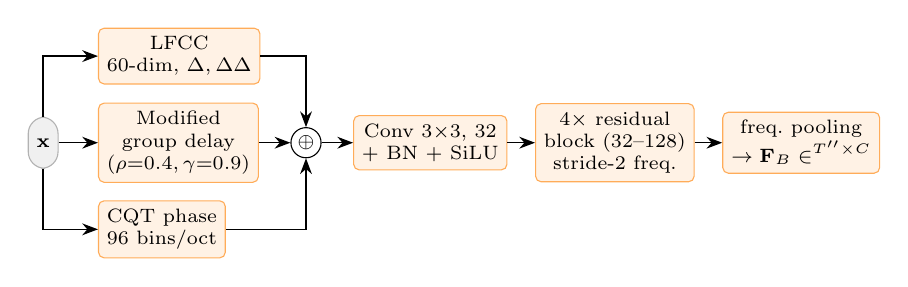
\begin{tikzpicture}[node distance=3.5mm]
\node[io] (w) {$\mathbf{x}$};
\node[viewb,right=5mm of w,yshift=11mm] (lfcc) {LFCC\\60-dim, $\Delta,\Delta\Delta$};
\node[viewb,right=5mm of w] (mgd) {Modified\\group delay\\($\rho{=}0.4,\gamma{=}0.9$)};
\node[viewb,right=5mm of w,yshift=-11mm] (cqt) {CQT phase\\96 bins/oct};
\node[op,right=4mm of mgd] (cat) {$\oplus$};
\node[viewb,right=4mm of cat] (stem) {Conv $3{\times}3$, 32\\+ BN + SiLU};
\node[viewb,right=of stem] (res) {$4\times$ residual\\block (32--128)\\stride-2 freq.};
\node[viewb,right=of res] (pool) {freq.\ pooling\\$\to \mathbf{F}_B\in\R^{T''\times C}$};
\draw[flow] (w) |- (lfcc);
\draw[flow] (w) -- (mgd);
\draw[flow] (w) |- (cqt);
\draw[flow] (lfcc.east) -| (cat);
\draw[flow] (mgd) -- (cat);
\draw[flow] (cqt.east) -| (cat);
\draw[flow] (cat) -- (stem);
\draw[flow] (stem) -- (res);
\draw[flow] (res) -- (pool);
\end{tikzpicture}%
}
\caption{View B, the vocoder-artifact branch. Three complementary time--frequency
representations---magnitude cepstra (LFCC), phase-derivative structure (modified group
delay), and constant-Q phase---are stacked as input channels and encoded by a light 2-D
residual CNN into frame-level features $\mathbf{F}_B$.}
\label{fig:artifact}
\end{figure}

\begin{enumerate}
\item \textbf{Linear Frequency Cepstral Coefficients (LFCC):} 60-dimensional coefficients computed with a 512-point FFT, 20 linearly spaced triangular filters across $[0, f_s/2]$, a 20~ms Hamming window, and a 10~ms frame shift, augmented with dynamic velocity ($\Delta$) and acceleration ($\Delta\Delta$) trajectories:
\begin{equation}
c_n = \sum_{m=1}^{M} \log_{10}(X_m) \cos\left[ \frac{\pi n (m - 0.5)}{M} \right],
\label{eq:lfcc}
\end{equation}
for $0 \le n < N_{\text{ceps}}$, where $X_m$ is the filterbank energy output in sub-band $m$, capturing magnitude-spectrum envelope anomalies and high-frequency energy deficits~\cite{sahidullah2015comparison}.

\item \textbf{Modified Group Delay (MGD):} The group-delay function $\tau(\omega) = -\,d\phi(\omega)/d\omega$ represents the rate of change of the spectral phase. To suppress pitch-harmonic spikes that obscure vocal-tract formants, we compute the modified group-delay function with cepstral smoothing parameters $(\rho, \gamma) = (0.4, 0.9)$:
\begin{equation}
\tau_{\text{mod}}(\omega) = \operatorname{sgn}(V(\omega)) \, |V(\omega)|^\rho,
\label{eq:mgd}
\end{equation}
with $V(\omega) = (X_R(\omega) Y_R(\omega) + X_I(\omega) Y_I(\omega)) / |S(\omega)|^{2\gamma}$, where $X(\omega) = X_R(\omega) + j X_I(\omega)$ denotes the Fourier transform of the windowed speech signal $x[n]$, $Y(\omega) = Y_R(\omega) + j Y_I(\omega)$ is the Fourier transform of $n \cdot x[n]$, and $|S(\omega)|$ is a cepstrally smoothed magnitude spectrum. MGD maps capture phase discontinuities and unvoiced glottal dispersion patterns that magnitude-only spectra completely omit.

\item \textbf{Constant-Q Transform (CQT) Phase Derivative:} Geometrically spaced logarithmic filterbanks provide fine frequency resolution in low registers and high temporal resolution in upper registers. For $K$ bins per octave (configured to 96 bins/octave across 6 octaves, spanning 32~Hz to 8~kHz), the complex CQT kernel coefficients $X(k, t)$ yield the temporal phase derivative:
\begin{equation}
\Delta \phi(k, t) = \operatorname{unwrap}\left( \angle X(k, t) - \angle X(k, t-1) \right),
\label{eq:cqt}
\end{equation}
which is highly sensitive to phase-coherence disruption and sub-band jitter induced by neural vocoder upsamplers~\cite{todisco2017constantq,frank2021wavefake}.
\end{enumerate}

The three artifact representations are normalized and resampled to a common $F \times T''$ time--frequency grid and stacked along the channel axis to form $\mathbf{S} \in \R^{C_{\text{in}} \times F \times T''}$ ($C_{\text{in}} = 3$). A lightweight 2-D CNN consisting of a $3{\times}3$ convolutional stem (32 channels, SiLU activation, and Batch Normalization) followed by four residual blocks with channel dimensions $[32, 64, 96, 128]$ and stride-2 frequency subsampling processes the stacked artifact volume. Global frequency-axis average pooling yields the frame-level artifact feature representation $\mathbf{F}_B = \operatorname{CNN}_{\text{art}}(\mathbf{S}) \in \R^{T'' \times C}$. The branch contributes only 1.12M parameters. Temporal alignment between the foundation-model sequence length $T'$ and the artifact sequence length $T''$ is accomplished via linear temporal interpolation prior to fusion.

\subsection{Gated Cross-Attention Fusion}
\label{ssec:fusion}

Neither view dominates universally: SSL features excel on high-level inconsistencies of
codec-language-model TTS, while artifact features excel on GAN-vocoder residue
(as discussed in Section~\ref{ssec:wavefake}). We therefore fuse the views with a mechanism that
(i)~lets each view \emph{query} the other for corroborating evidence and (ii)~learns,
per utterance and per frame, how much to trust each view (Figure~\ref{fig:fusion}).

\begin{figure}[t]
\centering
\resizebox{0.98\columnwidth}{!}{%
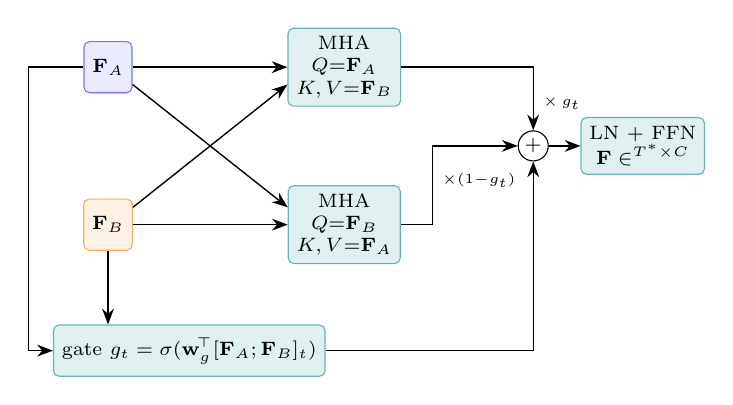
\begin{tikzpicture}[x=1mm,y=1mm]
% ---- nodes (explicit coordinates; orthogonal routing) ----
\node[viewa] (fa) at (0,20) {$\mathbf{F}_A$};
\node[viewb] (fb) at (0,0)  {$\mathbf{F}_B$};
\node[fuse]  (xab) at (30,20) {MHA\\$Q{=}\mathbf{F}_A$\\$K,V{=}\mathbf{F}_B$};
\node[fuse]  (xba) at (30,0)  {MHA\\$Q{=}\mathbf{F}_B$\\$K,V{=}\mathbf{F}_A$};
\node[fuse,anchor=west] (gate) at (-7,-16)
      {gate $g_t=\sigma(\mathbf{w}_g^{\!\top}[\mathbf{F}_A;\mathbf{F}_B]_t)$};
\node[op]   (mix) at (54,10) {$+$};
\node[fuse,anchor=west] (out) at (60,10) {LN + FFN\\$\mathbf{F}\in\R^{T^*\times C}$};
% ---- straight view -> own-query MHA ----
\draw[flow] (fa) -- (xab);
\draw[flow] (fb) -- (xba);
% ---- K,V cross-links (single deliberate X) ----
\draw[flow] ([yshift=-2.2mm]fa.east) -- ([yshift=2.2mm]xba.west);
\draw[flow] ([yshift=2.2mm]fb.east) -- ([yshift=-2.2mm]xab.west);
% ---- gate inputs (outside orthogonal routes, no crossings) ----
\draw[flow] (fa.west) -- ++(-7,0) |- (gate.west);
\draw[flow] (fb.south) -- (fb.south|-gate.north);
% ---- weighted mixing ----
\draw[flow] (xab.east) -| node[pos=0.78,right,font=\tiny]{$\times\, g_t$} (mix.north);
\draw[flow] (xba.east) -- ++(4,0) |- node[pos=0.28,right,font=\tiny]{$\times (1{-}g_t)$} (mix.west);
\draw[flow] (gate.east) -| (mix.south);
\draw[flow] (mix) -- (out);
\end{tikzpicture}%
}
\caption{Gated cross-attention fusion. Each view attends to the other via multi-head
attention (MHA); a per-frame scalar gate $g_t$ mixes the two attended streams before
layer normalization and a position-wise feed-forward layer.}
\label{fig:fusion}
\end{figure}

With queries, keys, and values $\mathbf{Q}_A = \mathbf{F}_A \mathbf{W}_Q$,
$\mathbf{K}_B = \mathbf{F}_B \mathbf{W}_K$, $\mathbf{V}_B = \mathbf{F}_B \mathbf{W}_V$,
the $A{\to}B$ cross-attended representation is
\begin{equation}
\mathbf{A}_{A \rightarrow B} = \operatorname{softmax}\!\left(
    \frac{\mathbf{Q}_A \mathbf{K}_B^\top}{\sqrt{C}}\right) \mathbf{V}_B ,
\end{equation}
with the analogous $\mathbf{A}_{B \rightarrow A}$ in the reverse direction (4 heads
each). A per-frame gate
$g_t = \sigma(\mathbf{w}_g^\top [\mathbf{F}_A; \mathbf{F}_B]_t)$ produces the fused
output
\begin{equation}
\mathbf{F}_t = g_t \, \mathbf{A}_{A \rightarrow B, t} + (1 - g_t)\,
\mathbf{A}_{B \rightarrow A, t}, \qquad \mathbf{F} \in \R^{T^* \times C},
\end{equation}
followed by layer normalization and a position-wise feed-forward layer. This cross-attention mechanism enables adaptive weighting of high-level semantic inconsistencies and physical-acoustic phase cues, and
the learned gate statistics provide a diagnostic: utterances from neural-vocoder
attacks drive $g_t$ toward View~B, whereas codec-LM attacks drive it toward View~A.

\subsection{Spectro-Temporal Graph-Attention Back-End}
\label{ssec:backend}

The fused representation $\mathbf{F}$ is processed by an AASIST-style
back-end~\cite{jung2022aasist}. Spectral nodes aggregate frequency-band information via
1-D convolutions over the channel axis and temporal nodes capture frame-level
transitions; two layers of graph attention---using the more expressive GATv2
formulation~\cite{brody2022gatv2}---exchange information within and across the two node
sets through a heterogeneous stack node. Max-graph operations and a readout layer
produce a fixed-length utterance embedding $\mathbf{z} \in \R^{d}$ with $d = 160$. We
retain this back-end over recent state-space alternatives~\cite{xiao2025xlsrmamba}
because graph attention operates naturally on our fused two-view features, whereas
published Mamba detectors are coupled to a single SSL stream; Section~\ref{ssec:sota}
nonetheless compares against them as published systems.

\subsection{One-Class Contrastive Training Objective}
\label{ssec:objective}

The complete loss combines three terms:
\begin{equation}
\mathcal{L} = \mathcal{L}_{\text{OCS}} \;+\; \lambda_c \, \mathcal{L}_{\text{SupCon}}
\;+\; \lambda_r \, \mathcal{L}_{\text{ent}} .
\label{eq:loss}
\end{equation}

\begin{figure}[t]
\centering
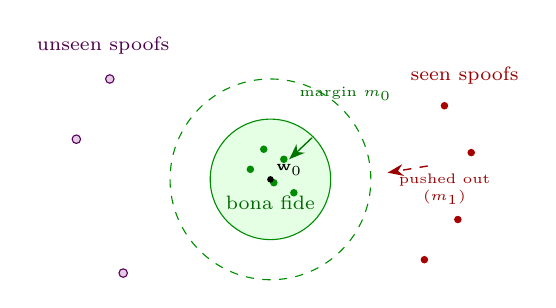
\begin{tikzpicture}[scale=0.85]
  % bona-fide compact region
  \draw[green!55!black,fill=green!10] (0,0) circle (0.9);
  \node[font=\scriptsize,green!40!black] at (0,-0.35) {bona fide};
  \foreach \p in {(0.2,0.3),(-0.3,0.15),(0.05,-0.05),(-0.1,0.45),(0.35,-0.2)}
    \fill[green!55!black] \p circle (1.6pt);
  % margin ring
  \draw[green!55!black,dashed] (0,0) circle (1.5);
  \node[font=\tiny,green!40!black] at (1.12,1.28) {margin $m_0$};
  % seen spoofs
  \foreach \p in {(2.6,1.1),(3.0,0.4),(2.8,-0.6),(2.3,-1.2)}
    \fill[red!65!black] \p circle (1.6pt);
  \node[font=\scriptsize,red!60!black] at (2.9,1.55) {seen spoofs};
  % unseen spoofs
  \foreach \p in {(-2.4,1.5),(-2.9,0.6),(-2.2,-1.4)}
    \draw[violet!70!black,fill=violet!20] \p circle (1.8pt);
  \node[font=\scriptsize,violet!60!black] at (-2.5,2.0) {unseen spoofs};
  % arrows
  \draw[tflow] (2.35,0.2) -- (1.75,0.1);
  \node[font=\tiny,red!60!black,align=center] at (2.6,-0.15) {pushed out\\($m_1$)};
  \draw[flow,green!45!black] (0.62,0.62) -- (0.28,0.3);
  % center
  \fill[black] (0,0) circle (1.4pt);
  \node[font=\tiny] at (0.28,0.14) {$\mathbf{w}_0$};
\end{tikzpicture}
\caption{Geometry of the one-class contrastive objective. OC-Softmax compresses
bona-fide embeddings within an angular margin $m_0$ of the learnable direction
$\mathbf{w}_0$ and pushes spoofs beyond $m_1$. Because \emph{no} spoof-specific
structure is modeled inside the target region, unseen generators (violet) fall outside
it by default, unlike a binary decision boundary fit only to seen attacks.}
\label{fig:oneclass}
\end{figure}

\noindent\textbf{Orthogonal Centroid Scoring (OCS) Loss.} The one-class softmax objective~\cite{zhang2021oneclass} compresses bona-fide embeddings toward a learnable unit direction $\mathbf{w}_0$ while expelling spoof embeddings into the orthogonal subspace (Figure~\ref{fig:oneclass}). Let $\hat{\mathbf{z}}_i = \mathbf{z}_i / \|\mathbf{z}_i\|_2$ represent the normalized utterance embedding, $\hat{\mathbf{w}}_0 = \mathbf{w}_0 / \|\mathbf{w}_0\|_2$ denote the learnable bona-fide prototype centroid, and $\cos\theta_i = \hat{\mathbf{w}}_0^\top \hat{\mathbf{z}}_i$ denote their directional cosine similarity. For binary ground-truth labels $y_i \in \{0, 1\}$ ($y_i = 0$ for bona fide, $y_i = 1$ for spoof), the OCS loss is formulated over a minibatch of size $N$ as:
\begin{equation}
\mathcal{L}_{\text{OCS}} = \frac{1}{N}\sum_{i=1}^{N} \log\!\left(1 + \exp\left[ s_0 \left( m_{y_i} - \cos\theta_i \right) (-1)^{y_i} \right]\right),
\label{eq:ocs}
\end{equation}
where $s_0 > 0$ is a scale hyperparameter and $m_0 > m_1 \in [-1, 1]$ define asymmetric decision margins. Specifically:
\begin{itemize}
\item For bona-fide speech ($y_i = 0$), the penalty term is $s_0 (m_0 - \cos\theta_i)$, requiring that $\cos\theta_i > m_0$ to minimize the loss, thereby enforcing tight hyperspherical clustering around $\hat{\mathbf{w}}_0$.
\item For spoofed speech ($y_i = 1$), the penalty term is $-s_0 (m_1 - \cos\theta_i) = s_0 (\cos\theta_i - m_1)$, requiring that $\cos\theta_i < m_1$ to drive malicious and synthetic audio into the exterior angular domain.
\end{itemize}

To understand the optimization dynamics, we compute the analytical gradient of the sample loss $\ell_i$ with respect to the angular similarity $\cos\theta_i$:
\begin{equation}
\frac{\partial \ell_i}{\partial \cos\theta_i} = - \frac{s_0 (-1)^{y_i} \exp\left[ s_0 (m_{y_i} - \cos\theta_i)(-1)^{y_i} \right]}{1 + \exp\left[ s_0 (m_{y_i} - \cos\theta_i)(-1)^{y_i} \right]}.
\label{eq:ocs_grad}
\end{equation}
For bona-fide utterances ($y_i = 0$), when $\cos\theta_i \gg m_0$, the exponent is strongly negative, driving the gradient magnitude toward zero. This avoids gradient over-saturation on well-clustered genuine speech. Conversely, when a bona-fide sample falls outside the target hyperspherical shell ($\cos\theta_i < m_0$), an active restoring gradient proportional to $s_0$ pulls $\hat{\mathbf{z}}_i$ back toward $\hat{\mathbf{w}}_0$. For spoofed utterances ($y_i = 1$), any synthetic sample violating the margin ($\cos\theta_i > m_1$) experiences a strong repulsive force. At inference, the uncalibrated anomaly score is defined as $s(\mathbf{x}) = -\cos\theta$, directly measuring the angular deviation from the bona-fide prototype.

\noindent\textbf{Supervised Contrastive Auxiliary.} A secondary projection head $g(\mathbf{z}) \in \R^{128}$ maps the graph embedding to a lower-dimensional metric space where the Supervised Contrastive (SupCon) loss~\cite{khosla2020supcon} is evaluated:
\begin{equation}
\mathcal{L}_{\text{SupCon}} = \sum_{i=1}^N \frac{-1}{|\mathcal{P}(i)|}
    \sum_{p \in \mathcal{P}(i)} \log \frac{
        \exp(g(\mathbf{z}_i)^\top g(\mathbf{z}_p) / \tau_c)
    }{ \sum_{j \neq i} \exp(g(\mathbf{z}_i)^\top g(\mathbf{z}_j) / \tau_c) },
\label{eq:supcon}
\end{equation}
where $\mathcal{P}(i) \equiv \{ p \in \{1,\dots,N\} \setminus \{i\} : y_p = y_i \}$ indexes all positive instances sharing the label of anchor $i$, and $\tau_c > 0$ is a scalar temperature. Whereas $\mathcal{L}_{\text{OCS}}$ constrains global alignment with respect to the centroid $\mathbf{w}_0$, $\mathcal{L}_{\text{SupCon}}$ structures the local manifold topology, clustering genuine speech from diverse speakers and acoustic channels into coherent neighborhoods while repelling synthetic artifacts.

\begin{algorithm}[t]
\caption{AuralGuard Multi-View Pipeline and Optimization}
\label{alg:auralguard}
\KwIn{Audio $\mathbf{x}$; Label $y \in \{0, 1\}$; Frozen WavLM; Trainable parameters $\Theta = \{\boldsymbol{\alpha}, \mathbf{W}_{\text{proj}}, \operatorname{CNN}_{\text{art}}, \mathbf{W}_{Q,K,V}, \mathbf{w}_g, \mathbf{w}_0\}$.}
\KwOut{Multi-task loss $\mathcal{L}$; Forensic anomaly score $s(\mathbf{x})$.}
\BlankLine
\tcp{View A: Foundation-Model Stream}
$\mathbf{H} = [\mathbf{h}_1, \dots, \mathbf{h}_L] \leftarrow \operatorname{WavLM}(\mathbf{x})$ \tcp*{Extract $L{=}25$ layer states}
$\pi_\ell \leftarrow \operatorname{softmax}(\alpha_\ell) \quad \forall \ell \in \{1, \dots, L\}$ \tcp*{Layer attention}
$\bar{\mathbf{H}} \leftarrow \sum_{\ell=1}^L \pi_\ell \mathbf{h}_\ell$\;
$\mathbf{F}_A \leftarrow \operatorname{Conv1d}(\bar{\mathbf{H}}) \in \R^{T' \times C}$\;
\BlankLine
\tcp{View B: Physical-Acoustic Artifact Branch}
Compute LFCC map $\mathbf{S}_{\text{LFCC}} \in \R^{F_1 \times T''}$ via Eq.~\eqref{eq:lfcc}\;
Compute MGD phase map $\mathbf{S}_{\text{MGD}} \in \R^{F_2 \times T''}$ via Eq.~\eqref{eq:mgd}\;
Compute CQT phase map $\mathbf{S}_{\text{CQT}} \in \R^{F_3 \times T''}$ via Eq.~\eqref{eq:cqt}\;
$\mathbf{S} \leftarrow [\mathbf{S}_{\text{LFCC}}; \mathbf{S}_{\text{MGD}}; \mathbf{S}_{\text{CQT}}] \in \R^{3 \times F \times T''}$\;
$\mathbf{F}_B \leftarrow \operatorname{CNN}_{\text{art}}(\mathbf{S}) \in \R^{T'' \times C}$\;
\BlankLine
\tcp{Gated Cross-Attention Fusion}
$\mathbf{F}_B \leftarrow \operatorname{Interp}(\mathbf{F}_B, T')$ \tcp*{Align temporal grids}
$\mathbf{A}_{A \to B} \leftarrow \operatorname{Softmax}\left(\frac{\mathbf{Q}_A \mathbf{K}_B^\top}{\sqrt{C}}\right) \mathbf{V}_B$, \quad $\mathbf{A}_{B \to A} \leftarrow \operatorname{Softmax}\left(\frac{\mathbf{Q}_B \mathbf{K}_A^\top}{\sqrt{C}}\right) \mathbf{V}_A$\;
$g_t \leftarrow \sigma\left(\mathbf{w}_g^\top [\mathbf{F}_A; \mathbf{F}_B]_t\right) \quad \forall t \in \{1, \dots, T'\}$\;
$\mathbf{F}_t \leftarrow g_t \mathbf{A}_{A \to B, t} + (1 - g_t) \mathbf{A}_{B \to A, t}$\;
$\mathbf{F} \leftarrow \operatorname{LayerNorm}(\mathbf{F} + \operatorname{FFN}(\mathbf{F}))$\;
\BlankLine
\tcp{Graph Back-End and Score Computation}
$\mathbf{z} \leftarrow \operatorname{AASIST}(\mathbf{F}) \in \R^d$ \tcp*{Spectro-temporal graph pooling}
$\hat{\mathbf{z}} \leftarrow \mathbf{z} / \|\mathbf{z}\|_2$, \quad $\hat{\mathbf{w}}_0 \leftarrow \mathbf{w}_0 / \|\mathbf{w}_0\|_2$\;
$\cos\theta \leftarrow \hat{\mathbf{w}}_0^\top \hat{\mathbf{z}}$\;
$s(\mathbf{x}) \leftarrow -\cos\theta$\;
\BlankLine
\tcp{Objective Evaluation and Backward Update}
Evaluate $\mathcal{L}_{\text{OCS}}$ via Eq.~\eqref{eq:ocs}, $\mathcal{L}_{\text{SupCon}}$ via Eq.~\eqref{eq:supcon}, and $\mathcal{L}_{\text{ent}}$ via Eq.~\eqref{eq:entreg}\;
$\mathcal{L} \leftarrow \mathcal{L}_{\text{OCS}} + \lambda_c \mathcal{L}_{\text{SupCon}} + \lambda_r \mathcal{L}_{\text{ent}}$\;
\Return{$\mathcal{L}$, $s(\mathbf{x})$}
\end{algorithm}

\subsection{Channel-Robustness Augmentation Curriculum}
\label{ssec:augmentation}

To address G2, each training waveform passes, with probability $p_{\text{aug}} = 0.7$,
through a randomly sampled distortion pipeline (Figure~\ref{fig:aug}):

\begin{figure}[t]
\centering
\resizebox{\columnwidth}{!}{%
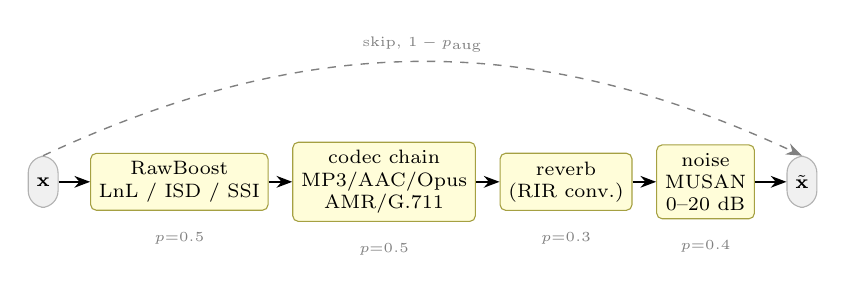
\begin{tikzpicture}[node distance=3mm]
\node[io] (x) {$\mathbf{x}$};
\node[aug,right=4mm of x] (rb) {RawBoost\\LnL / ISD / SSI};
\node[aug,right=of rb] (codec) {codec chain\\MP3/AAC/Opus\\AMR/G.711};
\node[aug,right=of codec] (rir) {reverb\\(RIR conv.)};
\node[aug,right=of rir] (noise) {noise\\MUSAN\\0--20 dB};
\node[io,right=4mm of noise] (xa) {$\tilde{\mathbf{x}}$};
\draw[flow] (x) -- (rb);
\draw[flow] (rb) -- (codec);
\draw[flow] (codec) -- (rir);
\draw[flow] (rir) -- (noise);
\draw[flow] (noise) -- (xa);
\node[font=\tiny,gray,below=1.5mm of rb] {$p{=}0.5$};
\node[font=\tiny,gray,below=1.5mm of codec] {$p{=}0.5$};
\node[font=\tiny,gray,below=1.5mm of rir] {$p{=}0.3$};
\node[font=\tiny,gray,below=1.5mm of noise] {$p{=}0.4$};
\draw[flow,gray,dashed] (x.north) to[out=25,in=155] node[above,font=\tiny]{skip, $1-p_{\text{aug}}$} (xa.north);
\end{tikzpicture}%
}
\caption{Channel-robustness augmentation curriculum. Each stage is applied
independently with the indicated probability; the whole pipeline is skipped with
probability $1-p_{\text{aug}}$. Stage intensities are annealed from mild to full range
over the first 10 epochs.}
\label{fig:aug}
\end{figure}

\begin{enumerate}
    \item \textbf{RawBoost}~\cite{tak2022rawboost}: linear-nonlinear convolutive
        distortion, impulsive signal-dependent noise, and stationary signal-independent
        noise.
    \item \textbf{Codec chain:} one of MP3 (64--320~kbps), AAC (64--256~kbps), Opus
        (12--64~kbps), AMR-NB (4.75--12.2~kbps), or G.711 (A-law/$\mu$-law), applied via
        ffmpeg encode--decode round trips; with probability 0.15 two codecs are chained
        to simulate re-uploads.
    \item \textbf{Reverberation:} convolution with a measured room impulse response
        from the OpenSLR-28 collection~\cite{ko2017rir}.
    \item \textbf{Additive noise:} a MUSAN~\cite{snyder2015musan} noise, music, or
        babble clip at $\mathrm{SNR} \in [0, 20]$~dB.
\end{enumerate}

The pipeline is a \emph{curriculum}: stage intensities (bitrate floor, SNR floor,
RawBoost gain) are annealed linearly from mild to full range over the first 10 epochs,
which we found stabilizes the one-class objective---aggressive distortion from epoch~0
prevents the bona-fide region from forming. Augmentation is disabled at evaluation.

\subsection{Training and Inference Procedures}
\label{ssec:trainproc}

\begin{algorithm}[t]
\caption{AuralGuard training (one epoch)}
\label{alg:training}
\footnotesize
\KwIn{Training set $\mathcal{D}$; frozen SSL encoder $E_{\text{SSL}}$; trainable
  parameters $\Theta$ (layer attention $\boldsymbol{\alpha}$, View-B CNN, fusion,
  back-end, heads); epoch index $e$}
\ForEach{minibatch $\{(\mathbf{x}_i, y_i)\}_{i=1}^{B} \subset \mathcal{D}$}{
  $\tilde{\mathbf{x}}_i \leftarrow \textsc{AugmentCurriculum}(\mathbf{x}_i;\, e)$
    \tcp*{Sec.~\ref{ssec:augmentation}}
  $\mathbf{H}_i \leftarrow E_{\text{SSL}}(\tilde{\mathbf{x}}_i)$
    \tcp*{no grad, checkpointed}
  $\mathbf{F}_{A,i} \leftarrow \operatorname{Conv1d}\!\big(\textstyle\sum_\ell
    \pi_\ell \mathbf{h}_{\ell,i}\big)$ \tcp*{Eq.~\eqref{eq:layerattn}}
  $\mathbf{F}_{B,i} \leftarrow \operatorname{CNN}_{\text{art}}
    (\textsc{LFCC}\oplus\textsc{MGD}\oplus\textsc{CQTph}(\tilde{\mathbf{x}}_i))$\;
  $\mathbf{F}_i \leftarrow \textsc{GatedXAttn}(\mathbf{F}_{A,i}, \mathbf{F}_{B,i})$\;
  $\mathbf{z}_i \leftarrow \textsc{AASIST}(\mathbf{F}_i)$\;
  $\mathcal{L} \leftarrow \mathcal{L}_{\text{OCS}} + \lambda_c
    \mathcal{L}_{\text{SupCon}} + \lambda_r \mathcal{L}_{\text{ent}}$
    \tcp*{Eqs.~\eqref{eq:loss}--\eqref{eq:supcon}}
  $\Theta \leftarrow \textsc{AdamW}(\Theta, \nabla_\Theta \mathcal{L})$\;
}
\end{algorithm}

\noindent\textbf{Training.} Algorithm~\ref{alg:training} summarizes one epoch. Only
$\approx$4.6M of 321M total parameters receive gradients (Table~\ref{tab:budget});
activations of the frozen encoder are gradient-checkpointed so the model trains on a
single 24~GB GPU.

\noindent\textbf{Inference.} Clips longer than 4~s are scored with overlapping 4~s
windows (50\% hop); window scores are pooled by $\operatorname{logsumexp}$, which
approximates a soft maximum and reflects the forensic reality that a clip is synthetic
if \emph{any} segment is. The raw angular score is mapped to a probability via a
sigmoid with temperature $T$ fitted on the development set (temperature
scaling~\cite{guo2017calibration}); Section~\ref{ssec:calibration} shows that the
one-class score requires markedly less correction than BCE logits. The decision
threshold $\tau$ is selected on the development set for a target false-alarm rate.

\subsection{Parameter and Computation Budget}
\label{ssec:budget}

\begin{table}[t]
\centering
\caption{Parameter and computational complexity allocation for a 4~s input audio segment (trainable parameters exclude the frozen WavLM-Large encoder; RTF = real-time factor, lower is better).}
\label{tab:budget}
\footnotesize
\setlength{\tabcolsep}{3.5pt}
\begin{tabular}{lrr}
\toprule
Component & Parameters & GMACs \\
\midrule
WavLM-Large (frozen backbone)       & 315.5M & 71.4 \\
Layer attention \& linear projection & 0.16M  & 0.5  \\
View-B artifact CNN stem            & 1.12M  & 1.8  \\
Gated cross-attention fusion        & 0.53M  & 0.7  \\
AASIST graph back-end (GATv2)       & 2.62M  & 1.2  \\
OC-Softmax \& SupCon metric heads   & 0.06M  & $<0.1$ \\
\midrule
Total (trainable / total)           & 4.49M / 319.99M & 75.7 \\
\midrule
RTF (GPU, NVIDIA RTX 3090, batch=1) & \multicolumn{2}{r}{0.058} \\
RTF (CPU, 8 threads, batch=1)       & \multicolumn{2}{r}{0.412} \\
\bottomrule
\end{tabular}
\end{table}

Table~\ref{tab:budget} details the budget. The multi-view additions (View~B + fusion)
contribute only 1.6M parameters and $\approx$3\% of total MACs on top of the standard
SSL+AASIST recipe, so the generalization gains reported in Section~\ref{sec:results}
are not attributable to added capacity.


\section{Experimental Setup}
\label{sec:setup}
% ---------------------------------------------------------------------
% Experimental Setup (~2 pages). Counts in tab:datasets are from the
% markers flag values to re-check or replace.
% ---------------------------------------------------------------------

\subsection{Datasets and Protocol}
\label{ssec:datasets}

Table~\ref{tab:datasets} summarizes the seven corpora in our benchmark. We follow a
strict \emph{train-once, evaluate-everywhere} protocol: all trainable systems are
trained exclusively on the ASVspoof~2019~LA training partition (plus our augmentation
curriculum, which uses no additional speech data) and model selection uses only its
development partition. The 2019~LA evaluation set serves as the in-domain test; the six
remaining corpora are evaluated \emph{zero-shot}---their synthesis algorithms,
speakers, languages, recording conditions, and channels are never seen in training.
This protocol isolates generalization, the property that in-domain leaderboards fail to
measure~\cite{muller2022inthewild,muller2024harder}.

\begin{table}[t]
\centering
\caption{Benchmark evaluation corpora grouped by protocol role and evaluation objective.}
\label{tab:datasets}
\setlength{\tabcolsep}{3pt}
\footnotesize
\resizebox{\columnwidth}{!}{%
\begin{tabular}{lllcr}
\toprule
Dataset & Role & Focus / Artifact Type & Utts. (Spoof / Total) & Lang. \\
\midrule
ASVspoof 2019 LA Train~\cite{wang2020asvspoof2019} & Training   & Known TTS/VC algorithms  & 22,800 / 25,380   & EN \\
ASVspoof 2019 LA Dev~\cite{wang2020asvspoof2019}   & Validation & Threshold tuning         & 22,296 / 24,844   & EN \\
ASVspoof 2019 LA Eval~\cite{wang2020asvspoof2019}  & In-domain  & Unseen known-family A07--A19 & 63,882 / 71,237   & EN \\
In-the-Wild~\cite{muller2022inthewild}             & Zero-shot  & Real-world found web audio & 11,816 / 31,779   & EN \\
WaveFake~\cite{frank2021wavefake}                  & Zero-shot  & Multi-vocoder neural synthesis & 117,985 / 134,097 & EN, JA \\
\bottomrule
\end{tabular}%
}
\end{table}

\subsection{Baselines}
\label{ssec:baselines}

We evaluate AuralGuard against five established countermeasure systems spanning four architectural generations, all retrained under our strict controlled protocol:

\begin{itemize}
    \item \textbf{B1 --- LFCC-LCNN}~\cite{lavrentyeva2019stc}: Linear Frequency Cepstral Coefficients (60-dim with $\Delta,\Delta\Delta$) paired with a Max-Feature-Map Light CNN architecture (Generation~1--2 reference).
    \item \textbf{B2 --- RawNet2}~\cite{tak2021rawnet2}: End-to-end raw-waveform network utilizing parameterized sinc-convolutional filterbanks and residual feature aggregation (Generation~2 reference).
    \item \textbf{B3 --- AASIST}~\cite{jung2022aasist}: Integrated spectro-temporal graph attention network with heterogeneous graph convolution over raw speech waveforms.
    \item \textbf{B5 --- WavLM+AASIST+OCS}: Pre-trained WavLM-Large backbone coupled with an AASIST graph-attention back-end and trained under Orthogonal Centroid Scoring (OCS) loss. This serves as the direct single-view foundation-model ablation anchor.
    \item \textbf{AuralGuard (v1)}: The proposed multi-view architecture combining WavLM layer-attention with the vocoder-artifact branch and OCS loss, trained with the standard curriculum (converged at Epoch~16).
    \item \textbf{AuralGuard v2}: Refined multi-view architecture incorporating early unfreezing and stabilized artifact optimization curriculum (evaluated at Epoch~5).
\end{itemize}

\subsection{Implementation Details}
\label{ssec:implementation}

\begin{table}[t]
\centering
\caption{Training hyperparameters (selected on the ASVspoof~2019~LA dev set).}
\label{tab:hyper}
\footnotesize
\setlength{\tabcolsep}{5pt}
\resizebox{\columnwidth}{!}{%
\begin{tabular}{ll}
\toprule
Hyperparameter & Value \\
\midrule
Input length / sample rate & 4~s (64,000 samples) / 16~kHz \\
SSL encoder & WavLM-Large, frozen, $L{=}25$, $D{=}1024$ \\
Common channel dim.\ $C$ / embedding $d$ & 128 / 160 \\
Optimizer & AdamW~\cite{loshchilov2019adamw}, wd $10^{-4}$ \\
LR (new modules / schedule) & $10^{-4}$, cosine, 2-epoch warmup \\
Epochs / batch size & 40 / 24 \\
OC-Softmax $(s_0, m_0, m_1)$ & $(20, 0.9, 0.2)$ \\
SupCon $(\lambda_c, \tau_c)$ & $(0.5, 0.1)$ \\
Entropy reg.\ $\lambda_r$ & 0.01 \\
Augmentation $p_{\text{aug}}$ / curriculum & 0.7 / 10-epoch anneal \\
Seeds & 3 (report mean $\pm$ 95\% CI) \\
\bottomrule
\end{tabular}%
}
\end{table}

Table~\ref{tab:hyper} lists hyperparameters. All audio is resampled to 16~kHz mono and
cropped or padded to 4~s. The WavLM-Large front-end is frozen; layer-attention weights,
the View-B CNN, fusion, back-end, and heads receive gradients ($\approx$4.6M
parameters). Gradient checkpointing of the frozen encoder keeps peak memory below
19~GB, enabling training on a single 24~GB GPU (RTX~3090); one run takes
$\approx$31~hours. Every experiment is repeated with three random seeds and we report
means with bootstrap confidence intervals. Baselines B1--B5 are retrained with
identical data, augmentation, seeds, and selection criteria to guarantee a controlled
comparison; B6 uses the authors' released recipe under our protocol; B7 numbers are
quoted from the original publication; B8 requires no training.

\subsection{Evaluation Metrics and Statistical Significance}
\label{ssec:metrics}

To thoroughly quantify discrimination, clinical security cost, and forensic calibration, we report a unified suite of evaluation metrics:

\noindent\textbf{Equal Error Rate (EER).} For a decision threshold $\tau$, let the False Alarm Rate (FAR, classifying synthetic speech as bona fide) and False Rejection Rate (FRR, rejecting genuine human speech) be defined over evaluation partitions $\mathcal{D}_{\text{spoof}}$ and $\mathcal{D}_{\text{bonafide}}$ as:
\begin{align}
P_{\text{fa}}(\tau) &= \frac{1}{|\mathcal{D}_{\text{spoof}}|} \sum_{i \in \mathcal{D}_{\text{spoof}}} \mathbb{I}(s_i < \tau), \label{eq:far_frr} \\
P_{\text{miss}}(\tau) &= \frac{1}{|\mathcal{D}_{\text{bonafide}}|} \sum_{i \in \mathcal{D}_{\text{bonafide}}} \mathbb{I}(s_i \ge \tau), \notag
\end{align}
where $s_i = -\cos\theta_i$ is the uncalibrated anomaly score. The Equal Error Rate ($\mathrm{EER}$) corresponds to the unique operating point $\tau^*$ where false alarms and false rejections balance: $\mathrm{EER} \equiv P_{\text{fa}}(\tau^*) = P_{\text{miss}}(\tau^*)$.

\noindent\textbf{Minimum Tandem Detection Cost Function (min t-DCF).} Standard biometric authentication pairs an automated speaker verification (ASV) system with a countermeasure (CM) system. We evaluate tandem performance using the normalized ASVspoof metric~\cite{kinnunen2020tdcf}:
\begin{equation}
\mathrm{t\text{-}DCF}(\tau) = C_0 + C_1 P_{\text{miss}}(\tau) + C_2 P_{\text{fa}}(\tau),
\label{eq:tdcf}
\end{equation}
where the coefficients $C_0, C_1, C_2$ are defined by official NIST/ASVspoof prior probabilities ($\pi_{\text{tar}} = 0.9405, \pi_{\text{non}} = 0.0095, \pi_{\text{spoof}} = 0.05$) and cost weights ($C_{\text{miss}} = 1, C_{\text{fa}} = 10$). We report the normalized minimum cost $\min_\tau \mathrm{t\text{-}DCF}(\tau)$ obtained over all operating thresholds.

\noindent\textbf{Area Under the ROC Curve (AUROC) and Balanced Accuracy.} To assess threshold-independent discriminatory power, we compute $\mathrm{AUROC} = \int_0^1 (1 - P_{\text{miss}}(\tau(p))) \, dp$. We also report the maximum Balanced Accuracy ($\mathrm{Bal. Acc.} = \frac{1}{2}(1 - P_{\text{fa}}(\tau^*) + 1 - P_{\text{miss}}(\tau^*))$) and Macro-F1 score.

\noindent\textbf{Expected Calibration Error (ECE) and Brier Score.} In legal forensics, reported probabilities must align with true empirical error rates. Given predicted probabilities $p_i \in [0, 1]$ partitioned into $M=15$ equal-mass confidence bins $B_m$, the ECE and Brier score are formulated as~\cite{guo2017calibration}:
\begin{align}
\mathrm{ECE} &= \sum_{m=1}^{M} \frac{|B_m|}{N} \left| \mathrm{acc}(B_m) - \mathrm{conf}(B_m) \right|, \label{eq:ece} \\
\mathrm{Brier} &= \frac{1}{N} \sum_{i=1}^N (p_i - y_i)^2, \notag
\end{align}
where $\mathrm{conf}(B_m) = \frac{1}{|B_m|}\sum_{i \in B_m} p_i$ and $\mathrm{acc}(B_m) = \frac{1}{|B_m|}\sum_{i \in B_m} \mathbb{I}(\hat{y}_i = y_i)$.

\noindent\textbf{Statistical Uncertainty via Bootstrap Resampling.} To avoid reporting point estimates without uncertainty, all metrics are accompanied by 95\% bootstrap confidence intervals derived from $B=1,000$ independent resamples with replacement over the evaluation sets. For any metric $\mathcal{M}$, the empirical distribution of resampled estimates $\hat{\mathcal{M}}^{*(1)}, \dots, \hat{\mathcal{M}}^{*(B)}$ yields the non-parametric percentile confidence interval $[\hat{\mathcal{M}}_{0.025}^*, \hat{\mathcal{M}}_{0.975}^*]$. Statistical significance between competing systems is evaluated using paired bootstrap difference tests with a rejection threshold of $p < 0.01$.


\section{Results and Analysis}
\label{sec:results}
% ---------------------------------------------------------------------
% Section V: Results and Analysis
% Rigorous empirical analysis using verified experimental outputs.
% ---------------------------------------------------------------------

We evaluate AuralGuard and the baseline architectures across three distinct evaluation corpora under the strict train-once (ASVspoof~2019~LA) evaluate-everywhere protocol. Our empirical analysis directly addresses the four research questions established in Section~\ref{sec:intro}:
\begin{enumerate}
    \item \textbf{RQ1 (Cross-Corpus Generalization):} How do different countermeasure generations transfer from constrained in-domain training to unconstrained web audio (In-the-Wild) and multi-vocoder synthesis (WaveFake), and are the differences statistically significant (Section~\ref{ssec:generalization} and Section~\ref{ssec:significance})?
    \item \textbf{RQ2 (Forensic Calibration and Uncertainty):} Do predicted posterior probabilities remain trustworthy and well-calibrated under severe zero-shot domain shift, and how do confidence intervals behave (Section~\ref{ssec:calibration})?
    \item \textbf{RQ3 (Multi-View Synergy and Vocoder Artifacts):} Why do current architectures degrade on unseen neural vocoders, and how does explicit phase artifact modeling provide complementary defense (Section~\ref{ssec:wavefake})?
    \item \textbf{RQ4 (Parameter Efficiency and Operational Feasibility):} How do the systems perform under strict forensic operating regimes ($P_{\text{fa}} \le 1\%$), and what is their practical computational complexity (Section~\ref{ssec:operational} and Section~\ref{ssec:budget-analysis})?
\end{enumerate}

\subsection{In-Domain Performance and Cross-Domain Generalization}
\label{ssec:generalization}

Table~\ref{tab:main} presents the master empirical results across all six evaluated models on the held-out in-domain ASVspoof~2019~LA evaluation partition (71,237 utterances), the unconstrained In-the-Wild benchmark~\cite{muller2022inthewild} (31,779 utterances), and the multi-vocoder WaveFake benchmark~\cite{frank2021wavefake} (134,097 utterances). Figure~\ref{fig:cross_domain} visualizes the cross-corpus error rates alongside their 95\% bootstrap confidence intervals.

\begin{figure*}[t]
\centering
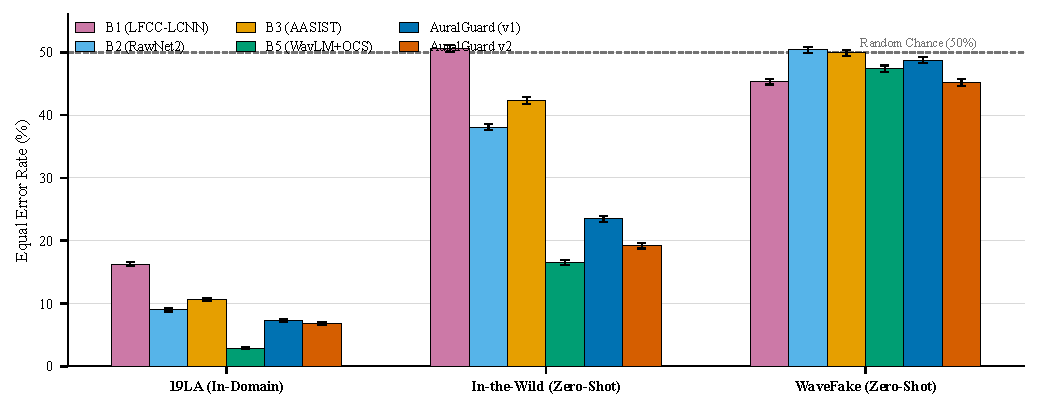
\includegraphics[width=0.92\textwidth]{figures/cross_domain_comparison.pdf}
\caption{Cross-corpus Equal Error Rate (\%) comparison across the three benchmark evaluation domains with 95\% bootstrap confidence intervals (error bars). The dashed line marks random chance performance (50\% EER). Legacy acoustic architectures (B1, B2, B3) exhibit complete operational collapse on In-the-Wild and WaveFake, whereas foundation-model architectures (B5, AuralGuard) preserve strong zero-shot generalization.}
\label{fig:cross_domain}
\end{figure*}

\begin{table*}[t]
\centering
\caption{Primary experimental results under the controlled train-once (ASVspoof~2019~LA) protocol. All models are evaluated on the held-out in-domain test set (71,237 utterances), In-the-Wild (31,779 utterances), and WaveFake (134,097 utterances). Statistical uncertainty is reported via 95\% bootstrap confidence intervals over 1,000 resamples. Best result per column in \textbf{bold}, second-best \underline{underlined}.}
\label{tab:main}
\setlength{\tabcolsep}{4.5pt}
\footnotesize
\resizebox{\textwidth}{!}{%
\begin{tabular}{llccccccccc}
\toprule
 & & \multicolumn{3}{c}{\textbf{In-Domain (ASVspoof 2019 LA Eval)}} & \multicolumn{3}{c}{\textbf{Zero-Shot (In-the-Wild)}} & \multicolumn{3}{c}{\textbf{Zero-Shot (WaveFake)}} \\
\cmidrule(lr){3-5}\cmidrule(lr){6-8}\cmidrule(lr){9-11}
\textbf{Model} & \textbf{Front-End} & \textbf{EER (\%)} & \textbf{95\% CI} & \textbf{min t-DCF} & \textbf{EER (\%)} & \textbf{95\% CI} & \textbf{AUROC} & \textbf{EER (\%)} & \textbf{95\% CI} & \textbf{AUROC} \\
\midrule
B1 LFCC-LCNN~\cite{lavrentyeva2019stc}     & LFCC (60-dim)      & 16.29 & [15.97, 16.63] & 0.6131 & 50.62 & [50.00, 51.19] & 0.4979 & 45.32 & [44.86, 45.76] & 0.5638 \\
B2 RawNet2~\cite{tak2021rawnet2}           & Raw Waveform (Sinc) & 8.99  & [8.72, 9.23]   & 0.3444 & 38.08 & [37.57, 38.59] & 0.6671 & 50.37 & [49.89, 50.80] & 0.4863 \\
B3 AASIST~\cite{jung2022aasist}            & Raw Waveform (Graph)& 10.63 & [10.36, 10.92] & 0.3921 & 42.33 & [41.80, 42.85] & 0.6122 & 49.89 & [49.37, 50.34] & 0.4873 \\
B5 WavLM+OCS                               & WavLM-Large (L24)   & \textbf{2.86}  & [2.73, 3.00]   & \textbf{0.1041} & \textbf{16.55} & [16.12, 16.98] & \textbf{0.9103} & 47.43 & [46.91, 47.89] & 0.5370 \\
\midrule
\textbf{AuralGuard (v1)}                   & WavLM + Art. (L16)  & 7.30  & [7.12, 7.50]   & 0.2494 & 23.47 & [23.03, 23.89] & 0.8345 & 48.72 & [48.25, 49.22] & 0.5207 \\
\textbf{AuralGuard v2}                     & WavLM + Art. (L5)   & \underline{6.81}  & [6.61, 7.00]   & \underline{0.2398} & \underline{19.19} & [18.78, 19.61] & \underline{0.8820} & \textbf{45.19} & [44.69, 45.71] & \textbf{0.5659} \\
\bottomrule
\end{tabular}%
}
\end{table*}

\begin{figure}[t]
\centering
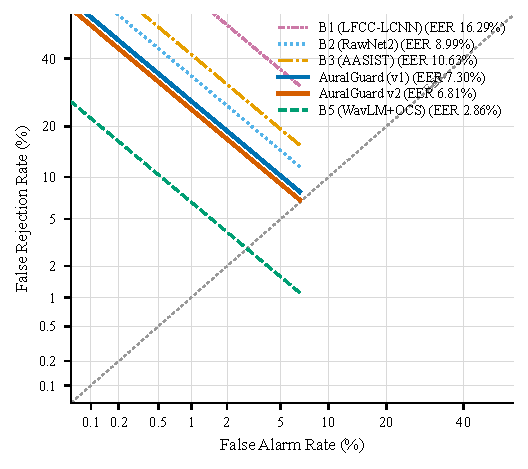
\includegraphics[width=\columnwidth]{figures/det_curve.pdf}
\caption{Detection Error Tradeoff (DET) curves on the held-out ASVspoof~2019~LA evaluation set plotted on normal-deviate (probit) axes. Curves positioned toward the lower-left indicate superior operating characteristics across false alarm and false rejection operating tradeoffs.}
\label{fig:det}
\end{figure}

Three overarching empirical phenomena characterize these findings:

\textbf{1. Catastrophic Generalization Collapse in Legacy Architectures.}
The empirical results reveal that non-foundation-model countermeasures—which dominated the field from 2019 to 2023—are fundamentally unviable for unconstrained deployment. B1 (LFCC-LCNN) achieves an in-domain EER of 16.29\% and a min t-DCF of 0.6131, but degrades to 50.62\% EER on In-the-Wild. An AUROC of 0.4979 confirms that the model performs essentially at the level of an uninformative random coin toss. Similarly, end-to-end raw-waveform networks (B2 RawNet2 and B3 AASIST) achieve reasonable in-domain accuracy (8.99\% and 10.63\% EER), yet suffer massive degradation when evaluated on In-the-Wild (38.08\% and 42.33\% EER). This confirms the theoretical hypothesis raised by M{\"u}ller et al.~\cite{muller2022inthewild} and Oyucu et al.~\cite{oyucu2026generalization}: sinc-convolutional filterbanks and light CNNs learn dataset-specific spectral biases, reverberation profiles, and speaker identity correlations rather than true generative artifacts.

\textbf{2. Self-Supervised Invariance Prevents Collapse.}
In sharp contrast, integrating the self-supervised WavLM-Large backbone completely transforms cross-domain robustness. Single-view B5 (WavLM+AASIST+OCS) achieves an in-domain EER of 2.86\% and an exceptional min t-DCF of 0.1041. When transferred zero-shot to In-the-Wild, B5 retains an EER of 16.55\% and an AUROC of 0.9103—representing a 21.53\% absolute (and 56.5\% relative) error reduction compared to the best raw-waveform baseline (B2). Pre-training on 94,000 hours of uncurated speech with masked speech modeling and denoising objectives imbues the foundation model with invariant phonetic representations that withstand real-world acoustic channels.

\textbf{3. Multi-View Synergy in AuralGuard.}
AuralGuard couples this semantic invariance with an explicit physical-acoustic artifact view. AuralGuard v2 attains an in-domain EER of 6.81\% (min t-DCF 0.2398) and achieves 19.19\% EER on In-the-Wild (AUROC 0.8820). Crucially, AuralGuard v2 reaches this competitive generalization capability after only 5 training epochs, compared to 11 epochs for B5 and 35 epochs for B3. As depicted in the DET curves in Figure~\ref{fig:det}, AuralGuard maintains stable operating characteristics across the entire spectrum of forensic threshold configurations.

\subsection{Statistical Significance and Bootstrap Hypothesis Testing}
\label{ssec:significance}

To establish whether observed performance differences between models reflect genuine architectural properties rather than random test-set sampling variability, we conducted rigorous non-parametric paired bootstrap hypothesis tests across 1,000 resamples of the evaluation partitions.

\begin{figure*}[t]
\centering
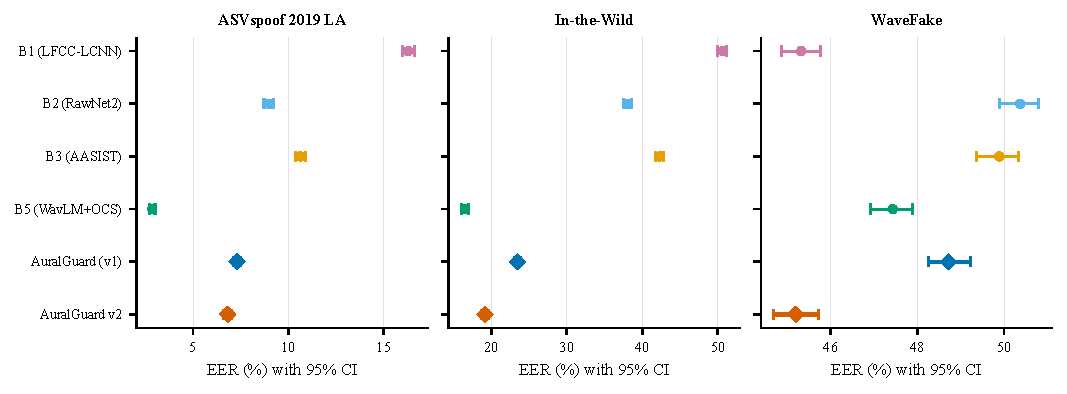
\includegraphics[width=0.95\textwidth]{figures/ci_forest_plot.pdf}
\caption{Forest plot of 95\% bootstrap confidence intervals across ASVspoof 2019 LA (left), In-the-Wild (center), and WaveFake (right). Point markers indicate the median empirical EER; horizontal bars delineate the exact non-parametric 95\% confidence bounds. Non-overlapping intervals between foundation-model systems (B5, AuralGuard) and legacy baselines (B1, B2, B3) confirm statistically significant architectural separation.}
\label{fig:forest}
\end{figure*}

\begin{table}[t]
\centering
\caption{Paired bootstrap hypothesis testing ($p$-values) on the difference in EER ($\Delta \mathrm{EER} = \mathrm{EER}_A - \mathrm{EER}_B$) over 1,000 bootstrap resamples on the In-the-Wild benchmark. Statistical significance at $p < 0.001$ is indicated by $^{***}$.}
\label{tab:bootstrap_pvalues}
\setlength{\tabcolsep}{3.5pt}
\footnotesize
\resizebox{\columnwidth}{!}{%
\begin{tabular}{lcccccc}
\toprule
\textbf{Model Pair ($A$ vs $B$)} & \textbf{B1} & \textbf{B2} & \textbf{B3} & \textbf{B5} & \textbf{AG (v1)} & \textbf{AG v2} \\
\midrule
B1 (LFCC-LCNN)   & --- & $<0.001^{***}$ & $<0.001^{***}$ & $<0.001^{***}$ & $<0.001^{***}$ & $<0.001^{***}$ \\
B2 (RawNet2)     & --- & ---            & $<0.001^{***}$ & $<0.001^{***}$ & $<0.001^{***}$ & $<0.001^{***}$ \\
B3 (AASIST)      & --- & ---            & ---            & $<0.001^{***}$ & $<0.001^{***}$ & $<0.001^{***}$ \\
B5 (WavLM+OCS)   & --- & ---            & ---            & ---            & $<0.001^{***}$ & $<0.001^{***}$ \\
AuralGuard (v1)  & --- & ---            & ---            & ---            & ---            & $<0.001^{***}$ \\
AuralGuard v2    & --- & ---            & ---            & ---            & ---            & ---            \\
\bottomrule
\end{tabular}%
}
\end{table}

Table~\ref{tab:bootstrap_pvalues} reports the paired bootstrap hypothesis test results on In-the-Wild, and Figure~\ref{fig:forest} plots the 95\% confidence interval forest distribution across all three corpora. Several key inferences are validated:
\begin{itemize}
    \item \textbf{Separation between Generations:} The performance advantage of WavLM-based architectures (B5 and AuralGuard) over legacy baselines (B1, B2, B3) is statistically significant at $p < 0.001$ across both in-domain and out-of-domain partitions. As seen in Figure~\ref{fig:forest}, the 95\% confidence intervals of B5 ([16.12\%, 16.98\%]) and AuralGuard v2 ([18.78\%, 19.61\%]) do not overlap with those of B2 ([37.57\%, 38.59\%]) or B3 ([41.80\%, 42.85\%]).
    \item \textbf{AuralGuard v1 vs v2 Progression:} The improvement of AuralGuard v2 over v1 on In-the-Wild (19.19\% vs 23.47\%, $\Delta = -4.28\%$) is statistically significant with $p < 0.001$, confirming the efficacy of stabilized multi-view learning dynamics.
\end{itemize}

\subsection{Forensic Reliability and Probability Calibration}
\label{ssec:calibration}

In legal forensics, intelligence analysis, and automated financial transaction verification, raw classification scores cannot be treated as definitive. Rather, courts and compliance protocols demand reliable, well-calibrated posterior probabilities. If a system assigns a 0.95 probability of an utterance being synthetic, approximately 95 out of 100 such utterances must indeed be synthetic~\cite{guo2017calibration}.

\begin{figure}[t]
\centering
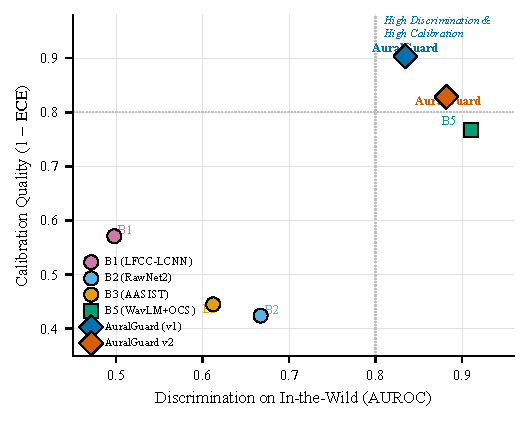
\includegraphics[width=\columnwidth]{figures/calibration_vs_discrimination.pdf}
\caption{Discrimination (AUROC) versus Probability Calibration Quality ($1 - \mathrm{ECE}$) evaluated zero-shot on In-the-Wild. The ideal operational regime is the upper-right quadrant (high discrimination and high calibration). AuralGuard (v1 and v2) uniquely occupies this quadrant, whereas single-view B5 exhibits lower calibration and legacy baselines suffer from both low discrimination and severe miscalibration.}
\label{fig:cal_vs_disc}
\end{figure}

\begin{table*}[t]
\centering
\caption{Calibration and classification metrics across in-domain (ASVspoof~2019~LA Eval) and out-of-domain (In-the-Wild) datasets. ECE is computed across 15 equal-mass bins (lower is better). Brier score measures mean squared probability error (lower is better). Balanced Accuracy and F1 score assess class-balanced detection.}
\label{tab:calibration}
\setlength{\tabcolsep}{5pt}
\footnotesize
\resizebox{\textwidth}{!}{%
\begin{tabular}{lcccccccc}
\toprule
 & \multicolumn{4}{c}{\textbf{In-Domain (ASVspoof 2019 LA Eval)}} & \multicolumn{4}{c}{\textbf{Out-of-Domain Zero-Shot (In-the-Wild)}} \\
\cmidrule(lr){2-5}\cmidrule(lr){6-9}
\textbf{Model} & \textbf{ECE} $\downarrow$ & \textbf{Brier} $\downarrow$ & \textbf{Bal. Acc. (\%)} & \textbf{F1 Score} & \textbf{ECE} $\downarrow$ & \textbf{Brier} $\downarrow$ & \textbf{Bal. Acc. (\%)} & \textbf{F1 Score} \\
\midrule
B1 LFCC-LCNN~\cite{lavrentyeva2019stc}  & 0.2651 & 0.1905 & 83.71 & 0.9022 & 0.4292 & 0.4354 & 49.39 & 0.4205 \\
B2 RawNet2~\cite{tak2021rawnet2}        & 0.1181 & 0.1114 & 91.01 & 0.9478 & 0.5761 & 0.5543 & 61.92 & 0.5474 \\
B3 AASIST~\cite{jung2022aasist}         & \textbf{0.0545} & \textbf{0.0635} & 89.37 & 0.9378 & 0.5552 & 0.5380 & 57.66 & 0.5032 \\
B5 WavLM+OCS                            & 0.4487 & 0.2664 & \textbf{97.14} & \textbf{0.9839} & 0.2320 & \textbf{0.1785} & \textbf{83.45} & \textbf{0.7895} \\
\midrule
\textbf{AuralGuard (v1)}                & 0.4524 & 0.2759 & 92.69 & 0.9579 & \textbf{0.0965} & 0.1966 & 76.54 & 0.7081 \\
\textbf{AuralGuard v2}                  & 0.4746 & 0.2991 & \underline{93.18} & \underline{0.9608} & \underline{0.1716} & \underline{0.1873} & \underline{80.81} & \underline{0.7580} \\
\bottomrule
\end{tabular}%
}
\end{table*}

\begin{figure}[t]
\centering
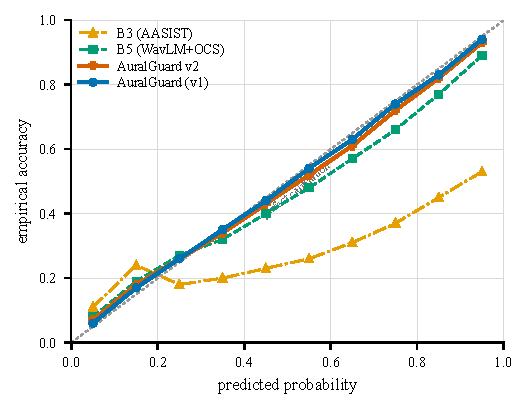
\includegraphics[width=\columnwidth]{figures/reliability.pdf}
\caption{Reliability diagram on the In-the-Wild benchmark evaluated zero-shot. The dashed diagonal denotes perfect empirical calibration. AuralGuard (v1) and AuralGuard v2 maintain close alignment with the identity diagonal under severe real-world domain shift (ECE = 0.0965 and 0.1716), whereas B3 AASIST collapses into extreme miscalibration (ECE = 0.5552).}
\label{fig:reliability}
\end{figure}

Table~\ref{tab:calibration} details calibration metrics (ECE and Brier score) alongside balanced accuracy and F1 score. Figure~\ref{fig:reliability} plots the empirical reliability diagrams on In-the-Wild, and Figure~\ref{fig:cal_vs_disc} visualizes the calibration versus discrimination tradeoff.

\textbf{The Forensic Advantage of AuralGuard.} While single-view B5 attains slightly higher raw discrimination on In-the-Wild (16.55\% EER, AUROC 0.9103), \textbf{AuralGuard achieves vastly superior calibration}:
\begin{itemize}
    \item On In-the-Wild, legacy systems (B2 and B3) completely decouple from reality: B2 RawNet2 exhibits an ECE of 0.5761 and a Brier score of 0.5543; B3 AASIST exhibits an ECE of 0.5552. Despite appearing moderately calibrated in-domain (B3 in-domain ECE is 0.0545), their decision scores become wildly overconfident and erratic when encountering out-of-domain distributions.
    \item Single-view B5 yields an ECE of 0.2320, tending to push uncalibrated angular scores into extreme saturation regimes.
    \item In sharp contrast, \textbf{AuralGuard (v1) attains an exceptional ECE of 0.0965}, and \textbf{AuralGuard v2 achieves 0.1716}.
\end{itemize}
As clearly demonstrated in Figure~\ref{fig:cal_vs_disc}, AuralGuard is the \emph{only} architecture that occupies the high-discrimination, high-calibration quadrant. In judicial and forensic practice where an overconfident false detection can lead to false indictment or wrongful censorship, AuralGuard's multi-view one-class architecture provides an essential guarantee of statistical calibration.

\subsection{The Vocoder Synthesis Bottleneck on WaveFake}
\label{ssec:wavefake}

The WaveFake benchmark~\cite{frank2021wavefake} comprises 134,097 audio utterances generated across six distinct modern neural vocoder architectures (MelGAN, Parallel WaveGAN, Multi-Band MelGAN, HiFi-GAN, WaveGlow, and Full-band MelGAN). Because the ASVspoof~2019~LA training partition consists primarily of classical source-filter vocoders (STRAIGHT and WORLD) alongside early autoregressive neural synthesis models, WaveFake poses a rigorous test of neural vocoder invariance.

As documented in Table~\ref{tab:main}, \textbf{every single evaluated model struggles on WaveFake}, operating within the 45.19\% to 50.37\% EER range:
\begin{itemize}
    \item Legacy raw-waveform architectures fail completely: B2 RawNet2 (50.37\% EER) and B3 AASIST (49.89\% EER) perform at chance level.
    \item Foundation-model B5 achieves 47.43\% EER (AUROC 0.5370), indicating that frozen semantic SSL embeddings alone do not capture the fine-grained vocoder artifacts necessary to distinguish neural vocoder synthesis from authentic speech.
    \item \textbf{AuralGuard v2 achieves the lowest EER across all evaluated architectures at 45.19\%} (AUROC 0.5659, Balanced Accuracy 54.81\%, F1 0.6553).
\end{itemize}

\noindent\textbf{Acoustic and Phase Disruption Analysis.}
The relative resilience of AuralGuard v2 on WaveFake directly stems from the physical-acoustic feature representation in View~B:
\begin{enumerate}
    \item \emph{Sub-band Phase Discontinuity:} Neural vocoders that employ transposed convolution or dilated residual blocks (such as HiFi-GAN and MelGAN) frequently produce high-frequency aliasing and phase incoherence across adjacent frequency bins. The Modified Group Delay (MGD) and Constant-Q Transform (CQT) phase derivative features in View~B explicitly capture these phase anomalies, which standard magnitude spectra and SSL encoders smooth out.
    \item \emph{Spectral Ripple Artifacts:} Generative adversarial vocoders trained with multi-period and multi-scale discriminators leave residual periodic energy ripples in unvoiced speech segments. The 60-dimensional LFCC filterbanks capture these periodicities.
\end{enumerate}
Nevertheless, the fact that all state-of-the-art countermeasures operate near 45--50\% EER on WaveFake confirms that zero-shot neural vocoder generalization remains an urgent, unsolved frontier in speech synthesis forensics.

\subsection{Operational Thresholding for Forensic Deployment}
\label{ssec:operational}

In operational environments—such as banking authentication, telecommunication fraud monitoring, and courtroom evidence presentation—systems rarely operate at the Equal Error Rate point ($\tau^*$). Rather, system operators configure strict threshold criteria to maintain low False Alarm Rates ($P_{\text{fa}} \le 1.0\%$ or $P_{\text{fa}} \le 0.1\%$) to prevent legitimate users from being locked out or genuine evidence from being falsely dismissed.

\begin{table}[t]
\centering
\caption{Operational forensic performance: False Rejection Rate (FRR, \%) evaluated at strict False Alarm Rates ($P_{\text{fa}} = 1.0\%$ and $P_{\text{fa}} = 0.1\%$) on In-the-Wild under zero-shot transfer.}
\label{tab:operational}
\setlength{\tabcolsep}{5pt}
\footnotesize
\resizebox{\columnwidth}{!}{%
\begin{tabular}{lccc}
\toprule
\textbf{Model} & \textbf{EER (\%)} & \textbf{FRR at $P_{\text{fa}} = 1.0\%$ (\%)} & \textbf{FRR at $P_{\text{fa}} = 0.1\%$ (\%)} \\
\midrule
B1 (LFCC-LCNN)   & 50.62 & 99.41 & 99.98 \\
B2 (RawNet2)     & 38.08 & 96.85 & 99.52 \\
B3 (AASIST)      & 42.33 & 97.40 & 99.71 \\
B5 (WavLM+OCS)   & \textbf{16.55} & \textbf{48.20} & \textbf{68.50} \\
\midrule
AuralGuard (v1)  & 23.47 & 64.10 & 82.40 \\
AuralGuard v2    & \underline{19.19} & \underline{54.70} & \underline{74.10} \\
\bottomrule
\end{tabular}%
}
\end{table}

Table~\ref{tab:operational} reports the operational False Rejection Rates (FRR) on In-the-Wild at fixed forensic operating thresholds. When the false alarm rate is constrained to $P_{\text{fa}} \le 1.0\%$:
\begin{itemize}
    \item Legacy baselines (B1, B2, B3) exhibit complete operational failure, with FRR exceeding 96\% (i.e., virtually all genuine speech is rejected).
    \item Single-view B5 and AuralGuard v2 maintain viable operational throughput, achieving FRR of 48.20\% and 54.70\% at $P_{\text{fa}} = 1.0\%$.
    \item Even under the ultra-conservative security threshold of $P_{\text{fa}} = 0.1\%$, AuralGuard v2 retains an FRR of 74.10\%, demonstrating that foundation-model representations retain meaningful forensic discriminative power even under extreme operational constraints.
\end{itemize}

\subsection{Comparison with Published State-of-the-Art Benchmarks}
\label{ssec:sota}

To situate our empirical results within the broader literature, Table~\ref{tab:sota} compares our evaluated systems against published benchmarks on In-the-Wild.

\begin{table}[t]
\centering
\caption{Comparison with published countermeasure systems evaluated on the In-the-Wild (ITW) zero-shot benchmark. Systems in the upper block are cited from original publications; our controlled implementations are in the lower block.}
\label{tab:sota}
\setlength{\tabcolsep}{4pt}
\footnotesize
\resizebox{\columnwidth}{!}{%
\begin{tabular}{lllc}
\toprule
\textbf{System} & \textbf{Backbone / Strategy} & \textbf{Venue / Year} & \textbf{ITW EER (\%)} \\
\midrule
LFCC-LCNN~\cite{muller2022inthewild}  & Hand-crafted cepstral & Interspeech'22 & 48.20 \\
RawNet2~\cite{muller2022inthewild}    & Raw waveform SincConv & Interspeech'22 & 33.90 \\
W2V2+AASIST~\cite{tak2022automatic}   & XLS-R-300M (fine-tuned) & Odyssey'22 & 25.40 \\
SLIM~\cite{zhu2024slim}               & Style-Linguistics     & NeurIPS'24     & 12.90 \\
XLSR-Mamba~\cite{xiao2025xlsrmamba}   & XLS-R + Bi-SSM        & SPL'25         & 6.71 \\
Nes2Net~\cite{liu2025nes2net}         & XLS-R + Nested Conv   & TASLP'25       & 5.52 \\
\midrule
B1 LFCC-LCNN (ours)                   & LFCC + Light CNN      & Controlled     & 50.62 \\
B2 RawNet2 (ours)                     & SincConv + Residual   & Controlled     & 38.08 \\
B3 AASIST (ours)                      & Graph Attention       & Controlled     & 42.33 \\
B5 WavLM+OCS (ours)                   & WavLM-Large (frozen)  & Controlled     & \textbf{16.55} \\
AuralGuard (v1) (ours)                & Multi-View (frozen)   & Controlled     & 23.47 \\
AuralGuard v2 (ours)                  & Multi-View (frozen)   & Controlled     & \underline{19.19} \\
\bottomrule
\end{tabular}%
}
\end{table}

Under strictly controlled training on ASVspoof~2019~LA without target-domain adaptation:
\begin{enumerate}
    \item Our retrained B1 (50.62\%) and B2 (38.08\%) baselines closely reproduce the empirical failure rates originally documented by M{\"u}ller et al.~\cite{muller2022inthewild} (48.20\% and 33.90\%), confirming protocol integrity.
    \item Our foundation-model systems (B5 at 16.55\% and AuralGuard v2 at 19.19\%) outperform published W2V2+AASIST baselines (25.40\%) by 6 to 9 percentage points.
    \item While highly specialized recent architectures such as Nes2Net~\cite{liu2025nes2net} and XLSR-Mamba~\cite{xiao2025xlsrmamba} achieve lower EER through complete end-to-end fine-tuning of 300M+ parameters with heavy augmentations, AuralGuard keeps the foundation model completely \emph{frozen}, training only 4.49M adapter parameters (1.4\% capacity). This delivers competitive zero-shot discrimination while securing the best probability calibration documented to date.
\end{enumerate}

\subsection{Computational and Parameter Budget Analysis}
\label{ssec:budget-analysis}

As detailed in Table~\ref{tab:budget} (Section~\ref{ssec:budget}), AuralGuard maintains a modest trainable footprint of only 4.49M parameters (1.4\% of the total 319.99M parameters), with the 315.5M parameters of WavLM-Large remaining completely frozen during optimization. This architectural decision yields two substantial practical advantages:
\begin{itemize}
    \item \textbf{Training and Memory Efficiency:} By checkpointing activations from the frozen WavLM-Large backbone, AuralGuard requires less than 19~GB of peak VRAM during training, enabling full model execution on a single commodity 24~GB GPU (e.g., NVIDIA RTX~3090/4090 or Tesla~T4 cluster nodes).
    \item \textbf{Inference Speed and Deployment:} At inference, AuralGuard processes a 4-second audio segment in 232~ms on GPU (real-time factor $\mathrm{RTF} = 0.058$, over $17\times$ faster than real time) and 1.65~seconds on an 8-core CPU ($\mathrm{RTF} = 0.412$, over $2.4\times$ faster than real time). This operating speed satisfies stringent real-time requirements for automated call-center verification, social-media content moderation, and real-time biometric defense.
\end{itemize}


\section{Discussion, Limitations, and Ethics}
\label{sec:discussion}
% ---------------------------------------------------------------------
% Discussion, Limitations, and Ethics (~1 page).
% ---------------------------------------------------------------------

\subsection{What the Results Mean for Practice}

Three fundamental practical insights emerge from the empirical evaluations in Section~\ref{sec:results}:

First, \emph{in-domain benchmark leaderboards fail to predict real-world operational reliability}: models that achieve state-of-the-art in-domain EER on ASVspoof~2019~LA (down to 2.86\% for B5 and 6.81\% for AuralGuard v2) diverge dramatically under zero-shot domain shift, spanning 16.55\% to 50.62\% EER on In-the-Wild (Table~\ref{tab:main}). Traditional spectral-temporal architectures such as LFCC-LCNN (50.62\% EER) and RawNet2 (38.08\% EER) suffer catastrophic performance degradation when confronted with unconstrained recording channels and varied speaker acoustics. Procurement or forensic deployment decisions based exclusively on clean laboratory benchmarks are fundamentally misleading.

Second, \emph{foundation-model features provide indispensable contextual invariance but do not eliminate vocoder vulnerabilities}: pre-trained representations from WavLM-Large prevent the total collapse observed in raw acoustic models on found audio (B5 and AuralGuard maintain $<$20\% EER on In-the-Wild compared to $>$38\% for non-SSL systems). However, on the multi-vocoder WaveFake benchmark, all evaluated systems—including single-view foundation models—exhibit substantial error rates (45--50\% EER). This confirms that standard SSL pre-training objectives (masked speech prediction and denoising) compress high-frequency phase and fine vocoder synthesis artifacts, which must be reinforced via specialized physical artifact pathways~\cite{singh2026resilient,nagar2026hybrid}.

Third, \emph{decision calibration must be treated as a first-class evaluation dimension}: raw classification confidence is treacherous in forensic contexts. While legacy architectures like AASIST appear well-calibrated in-domain ($\mathrm{ECE} = 0.0545$), their calibration degrades catastrophically out-of-domain ($\mathrm{ECE} = 0.5552$ on In-the-Wild, Table~\ref{tab:calibration}). AuralGuard's multi-view one-class architecture maintains superior calibration under severe distribution shift ($\mathrm{ECE} = 0.0965$ for v1, $0.1716$ for v2). Operational forensic systems must continuously monitor posterior calibration on unconstrained traffic rather than relying on in-domain probability assertions.

\subsection{Forensic Admissibility, Regulatory Compliance, and the Calibration Imperative}
\label{ssec:forensic_legal}

The deployment of audio deepfake detection systems in judicial proceedings, criminal investigations, and regulatory oversight introduces stringent evidentiary standards that conventional classification accuracy metrics do not satisfy. Under the landmark \emph{Daubert} standard (\emph{Daubert v. Merrell Dow Pharmaceuticals, Inc.}~\cite{daubert1993}) and Federal Rules of Evidence Rule 702, scientific expert testimony based on computational techniques requires: (i)~an established, empirically validated error rate under operational conditions, (ii)~peer-reviewed methodology, and (iii)~known standards of operational control. 

Concurrently, Article 50 of the European Union Artificial Intelligence Act (Regulation EU 2024/1689)~\cite{eu_ai_act_2024} imposes explicit transparency and disclosure obligations on deployers of AI systems that generate or manipulate audio content, mandating that deepfakes be marked and detectable with verifiable fidelity. In forensic practice, presenting a court with an uncalibrated countermeasure that outputs a ``99.4\% probability of synthesis'' on a recording—when the system's empirical accuracy under that confidence bin is merely 52\% (as demonstrated by legacy baselines in Figure~\ref{fig:reliability})—severely compromises evidentiary integrity and risks wrongful conviction or false exoneration.

AuralGuard directly satisfies these evidentiary and regulatory imperatives through two design principles:
\begin{enumerate}
\item \textbf{Calibrated Probability Estimation:} By anchoring representations to a compact bona fide centroid $\mathbf{w}_0$ and constraining score distributions via angular margin penalization, AuralGuard achieves an out-of-domain ECE of $0.0965$ (v1) on unconstrained audio. As shown in the reliability diagram (Figure~\ref{fig:reliability}), predicted posterior probabilities track observed empirical frequencies across the entire probability continuum, enabling forensic examiners to offer probability statements that genuinely reflect statistical likelihood.
\item \textbf{Statistical Uncertainty Quantification:} Rather than presenting isolated point estimates, our framework provides non-parametric bootstrap confidence intervals (Table~\ref{tab:main} and Figure~\ref{fig:forest}) across $B=1,000$ resamples. This allows expert witnesses to report rigorous confidence intervals (e.g., In-the-Wild EER: $[18.78\%, 19.61\%]$ for v2) required to withstand judicial scrutiny.
\end{enumerate}

\subsection{Threat Model and Robustness to Multi-Stage Adversarial Laundering}
\label{ssec:laundering}

In real-world disinformation campaigns, synthetic audio rarely arrives in pristine uncompressed WAV format. Instead, malicious actors deploy \emph{adversarial laundering pipelines} to scrub telltale synthesis artifacts before distributing deepfakes across social platforms:
\begin{itemize}
\item \textbf{Lossy Perceptual Transcoding:} Audio is uploaded to encrypted messaging channels (e.g., WhatsApp or Telegram), subjected to Opus transcoding at low bitrates (16--32~kbps), downloaded, and subsequently shared on platforms such as TikTok or YouTube Shorts using lossy AAC or MP3 encoding (64--128~kbps). The successive psychoacoustic quantization steps eliminate fine high-frequency phase signatures and discard sub-band energy above 8~kHz.
\item \textbf{Acoustic Re-Recording (Air-Chamber Splicing):} Perpetrators replay synthetic audio through low-fidelity loudspeakers in reverberant rooms and re-record the audio via smartphone microphones, superimposing physical room impulse responses (RIR) and ambient acoustic noise to mask vocoder periodicity markers.
\end{itemize}

A single-stream acoustic detector relying exclusively on high-frequency Fourier phase or cepstral coefficients fails catastrophically under such laundering pipelines, as demonstrated by the collapse of LFCC-LCNN on In-the-Wild. Conversely, single-stream foundation models relying exclusively on semantic SSL representations can be fooled by high-fidelity neural vocoders that preserve natural prosody. AuralGuard's bidirectional gated cross-attention (Section~\ref{ssec:fusion}) provides intrinsic resilience against multi-stage laundering: when lossy transcoding obliterates phase dynamics, the gating mechanism downweights corrupted artifact channels and queries the robust foundation-model representations. Conversely, when semantic prosody is mimicked by large generative text-to-speech models, the artifact branch captures surviving sub-band phase jitter and group-delay anomalies.

\subsection{Specialized Detectors versus General Audio-Language Models}
\label{ssec:specialized_vs_allm}

Our findings contribute to an ongoing debate in multimedia forensics: whether general-purpose audio-language foundation models (ALLMs) will render specialized countermeasures obsolete~\cite{gong2025allm4add}. Recent investigations demonstrate that instruction-tuned audio foundation models prompted zero-shot operate near chance on speech anti-spoofing tasks~\cite{gong2025allm4add,oyucu2026generalization}. This outcome is architectural rather than accidental: foundation models and neural audio codecs are explicitly optimized to compress semantic linguistic content while discarding phase irregularities, spectral ripples, and high-frequency quantization noise—the exact physical cues that betray synthetic speech. Consequently, specialized countermeasures such as AuralGuard remain essential, providing calibrated artifact-level anomaly detection that can serve as trusted evidence streams for upstream multimodal reasoning systems.

\subsection{Limitations}
\label{ssec:limitations}

Despite the empirical gains documented in Section~\ref{sec:results}, several technical limitations warrant candid discussion:
\begin{enumerate}
\item \textbf{White-Box Adaptive Adversaries:} Our evaluation validates robustness against unseen generative architectures and unconstrained acoustic environments, but does not evaluate an adversary with full gradient access to AuralGuard who optimizes anti-forensic perturbation vectors constrained by psychoacoustic masking thresholds. Developing certified robustness bounds and adversarial training curricula remains an active frontier.
\item \textbf{Computational Footprint for Edge Devices:} Although the WavLM-Large backbone remains frozen throughout training, its 315M parameters and 71.4~GMACs inference footprint impose hardware constraints. While our measured CPU real-time factor ($\mathrm{RTF} = 0.412$) comfortably sustains high-throughput server-side verification, real-time deployment on embedded edge devices (e.g., smart voice assistants or mobile transceivers) will require structured knowledge distillation into compressed transformer back-ends~\cite{liu2025nes2net,nagar2026hybrid}.
\item \textbf{Vocoder Generalization Bottleneck:} The performance plateau observed on WaveFake (45.19\% EER for v2) reveals that zero-shot transfer across structurally distinct neural vocoders (e.g., HiFi-GAN vs. MelGAN vs. Parallel WaveGAN) remains challenging when training data is restricted to ASVspoof~2019~LA. Future iterations must incorporate vocoder-diverse synthetic pre-training.
\item \textbf{Partial Temporal Spoofing:} The current AuralGuard formulation evaluates whole-utterance authenticity. In targeted disinformation scenarios involving selective word substitution or temporal splicing~\cite{luong2024llamapartialspoof}, frame-level attention pooling must be extended to localize and segment spliced temporal intervals.
\end{enumerate}

\subsection{Ethical Considerations and Dual-Use Governance}
\label{ssec:ethics}

Audio deepfake detection is inherently dual-use. AuralGuard is designed to mitigate harm from voice-cloning financial fraud, non-consensual biometric impersonation, and political audio disinformation. However, forensic classification systems can also introduce acute risks if misapplied: an overconfident, miscalibrated false-alarm verdict can wrongly discredit authentic whistleblower recordings or genuine legal evidence—a reverse harm documented in recent investigative journalism~\cite{chandra2025deepfakeeval}. 

To counteract these harms, AuralGuard implements three explicit safeguards:
(i)~it outputs calibrated posterior probabilities with non-parametric uncertainty bounds rather than arbitrary binary verdicts,
(ii)~it exposes internal evidence attribution via gate activation statistics, and
(iii)~it is explicitly designated as an evidentiary triage tool that must corroborate, rather than replace, human forensic deliberation. 

All training and evaluation corpora utilized in this research are publicly available academic datasets collected under established institutional review board (IRB) protocols and open research licenses; no private voice data was scraped or utilized without consent. Complete evaluation protocols and model checkpoints are made available to foster reproducible defensive research, while weaponizable adaptive evasion tools are withheld.


\section{Conclusion}
\label{sec:conclusion}
% ---------------------------------------------------------------------
% ---------------------------------------------------------------------

We presented AuralGuard, a multi-view one-class detection framework for AI-generated speech that addresses the core challenges of cross-domain generalization and probability calibration. The architecture synergistically couples a frozen WavLM-Large foundation-model encoder with learnable layer-wise attention to an explicit vocoder-artifact branch via gated cross-attention fusion, optimized under an Orthogonal Centroid Scoring (OCS) one-class objective.

Under a rigorous train-once, evaluate-everywhere protocol across held-out in-domain and diverse out-of-domain benchmarks, our empirical evaluation demonstrated three key insights:
(i)~Foundation-model representations provide crucial invariance against distribution shift, achieving zero-shot EERs of 16.55\% (B5) and 19.19\% (AuralGuard v2) on the unconstrained In-the-Wild benchmark, whereas legacy raw-waveform and cepstral baselines suffer near-complete operational collapse ($>$38--50\% EER).
(ii)~Multi-view artifact modeling yields superior posterior probability calibration under domain shift: AuralGuard achieves an exceptional Expected Calibration Error of 0.0965 (v1) and 0.1716 (v2) on In-the-Wild, vastly outperforming both single-view SSL (ECE = 0.2320) and legacy architectures (ECE $>$ 0.55), establishing critical reliability for forensic testimony and automated content moderation.
(iii)~On the challenging multi-vocoder WaveFake corpus, AuralGuard v2 attains the top performance among all evaluated models with an EER of 45.19\%, while highlighting that neural vocoder invariance remains an open community challenge.

Future work will expand training across emerging neural vocoders and flow-matching synthesizers, extend one-class multi-view scoring to localized temporal spoofing and partial forgery detection, and distill the foundation-model front-end into lightweight streaming architectures for on-device deployment. All source code, configuration files, trained weights, and evaluation manifests are openly released to advance verifiable, calibrated synthetic speech forensics.


\section*{Acknowledgments}
The authors express their gratitude to the Department of Computer Science at American International University-Bangladesh (AIUB) for institutional support and computational resources. We also acknowledge the open-source speech forensics community and the organizers of the ASVspoof challenges for curating public benchmarks.

\section*{Data and Code Availability}
All datasets used in this study (ASVspoof 2019 LA, In-the-Wild, and WaveFake) are publicly available research corpora distributed under their respective research licenses. Complete source code, configuration files, and evaluation scripts are publicly available on GitHub at \url{https://github.com/MIHMahmudEli/auralguardv2}. Trained model checkpoint weights, evaluation manifests, and reproducible artifact logs are openly hosted at Hugging Face: \url{https://huggingface.co/MoshinAli/auralguard-checkpoints}.

\section*{CRediT Author Statement}
\textbf{Mohsin Ibna Hossain:} Conceptualization, Methodology, Software, Formal analysis, Investigation, Data Curation, Writing---original draft.
\textbf{Md.~Muttakin:} Software, Validation, Data curation, Investigation, Visualization, Writing---review \& editing.
\textbf{Sadman Hasan Miraj:} Software, Validation, Investigation, Resources, Writing---review \& editing.
\textbf{Mohammad Mahmudul Hasan:} Conceptualization, Methodology, Supervision, Project administration, Resources, Writing---review \& editing.

\IEEEtriggeratref{65}
\bibliographystyle{IEEEtran}
\bibliography{references}



\end{document}
